
\documentclass[12pt]{article}


\usepackage{bbm}
\usepackage{float}
\usepackage{caption, subcaption}
\usepackage[T1]{fontenc}
\usepackage{url}
\usepackage[utf8]{inputenc}
\usepackage{booktabs} % For prettier tables
\usepackage{siunitx} % For aligning numbers at the decimal point
\usepackage{caption} % For captions
\usepackage{amsmath}
\usepackage{graphicx}
\usepackage{subcaption}
\usepackage{setspace}
\usepackage{graphicx}
\usepackage{subcaption}
\usepackage{amssymb}
\graphicspath{{Images/}}
\usepackage{parskip}
\usepackage{multirow}
\usepackage{enumitem}
\usepackage{amssymb}

\usepackage[backend=bibtex, maxbibnames=99, sorting=none, style=authoryear]{biblatex}
\addbibresource{sample.bib}


\usepackage{framed}
\usepackage{fancyhdr}
\usepackage{vmargin}
\usepackage{subcaption} %usamos subcaption mejor que subfig (más moderno)
\usepackage{eurosym}
\usepackage[table,xcdraw]{xcolor} % add color to your tables
\usepackage[bottom]{footmisc} %footnotes
\definecolor{blau}{RGB}{210,235,255}
\definecolor{blau2}{RGB}{120,170,225}
\setmarginsrb{2.5 cm}{2 cm}{2 cm}{2.5 cm}{1 cm}{0.5 cm}{1 cm}{1 cm}

\usepackage{multirow}

\usepackage{chngcntr}

\usepackage[framed, numbered]{matlab-prettifier}
 
\counterwithin{figure}{section}
\counterwithin{table}{section}
\numberwithin{equation}{section}

\usepackage{titlesec}
\usepackage{hyperref}
\usepackage{listings}
\usepackage{multicol}
\setlength{\columnsep}{1cm}

\titleclass{\subsubsubsection}{straight}[\subsection]

\newcounter{subsubsubsection}[subsubsection]
\renewcommand\thesubsubsubsection{\thesubsubsection.\arabic{subsubsubsection}}
\renewcommand\theparagraph{\thesubsubsubsection.\arabic{paragraph}} % optional; useful if paragraphs are to be numbered

\titleformat{\subsubsubsection}
  {\normalfont\normalsize\bfseries}{\thesubsubsubsection}{1em}{}
\titlespacing*{\subsubsubsection}
{0pt}{3.25ex plus 1ex minus .2ex}{1.5ex plus .2ex}

\makeatletter
\renewcommand\paragraph{\@startsection{paragraph}{5}{\z@}%
  {3.25ex \@plus1ex \@minus.2ex}%
  {-1em}%
  {\normalfont\normalsize\bfseries}}
\renewcommand\subparagraph{\@startsection{subparagraph}{6}{\parindent}%
  {3.25ex \@plus1ex \@minus .2ex}%
  {-1em}%
  {\normalfont\normalsize\bfseries}}
\def\toclevel@subsubsubsection{4}
\def\toclevel@paragraph{5}
\def\toclevel@paragraph{6}
\def\l@subsubsubsection{\@dottedtocline{4}{7em}{4em}}
\def\l@paragraph{\@dottedtocline{5}{10em}{5em}}
\def\l@subparagraph{\@dottedtocline{6}{14em}{6em}}
\makeatother

\usepackage[table,xcdraw]{xcolor}

\setcounter{secnumdepth}{4}
\setcounter{tocdepth}{4}


\usepackage{pdflscape} %Per poder posar la pàgina en horizontal
\usepackage{multicol} %Escriure en columnes 
 
	% Author
\date{\today}							% Date

\makeatletter
\let\thetitle\@title
\let\theauthor\@author
\let\thedate\@date
\makeatother

\pagestyle{fancy}
\fancyhf{}
\lhead{Networks: Concepts and Algorithms}
\rhead{Movie Recommendation Systems Using Networks}
\cfoot{\thepage}

\begin{document}

\begin{titlepage}
	\centering
    
\includegraphics[scale = 0.7]{bse_logo.png}\\[1.2 cm]	% University Logo
    \textsc{\LARGE Barcelona School of Economics}\\[2.0 cm]	% University Name
	\textsc{\Large Data Science Methodology Program}\\[0.5 cm]				% Course Code
	\textsc{\large 21D009 Networks: Concepts and Algorithms }\\[0.5 cm]				% Course Name
	\rule{\linewidth}{0.2 mm} \\[0.4 cm]
	{ \huge \bfseries Movie Recommendation Systems Using Networks}\\
	\rule{ \linewidth}{0.2 mm} \\[1.5 cm]
	
\begin{center}
    
{ \emph{Authors: }\\
    \textsc{Codd}, Jonny \\
    \textsc{Chen}, Joshua \\
    \textsc{Gallegos}, Rafael \\
    \textsc{Pérez}, Carlos \\ } 

\vspace{0.7cm}


    \textit{Professors:}\\  \textsc{Milán}, Pau \\
    	\textsc{Komander}, Björn
        \\ \vspace{0.5cm}


\vspace{1.7cm}


{\large December $20^{th}$, 2023} \\[2 cm]

 \end{center}
	\vfill
	
\end{titlepage}
	
\vspace{1cm}
\pagebreak

\newpage

\section{Introduction}

With the increase in choice across various domains, from entertainment to online social networks, recommendation systems have become increasingly crucial in alleviating information overload and shaping experience in every-day life. This has fueled demand for ever more sophisticated methods to delivery personalised recommendations as the variety of choice continues to expand. Historically, personal recommendations were primarily sourced from one's social circles, operating on the premise that friends or acquaintances with similar interests or tastes could offer valuable suggestions. This traditional approach, while effective to a degree, was inherently limited by the scope of one's immediate social network. However, modern recommendations systems now operate and build on a similar premise, leveraging network and network-adjacent concepts to understand the connections between people and tailor recommendations to individuals preference.

Currently, as we see recommendation systems utilize advancements in machine/deep learning to become more powerful and precise, we are furthering conversations on the increasingly central role that these recommendations systems take on shaping people's preferences. In some sense, recommendation algorithms have gotten so good that, instead of trying their best to predict consumer preferences, they are now creating consumer preferences. 

Our project is two-fold. Using the concepts learned in this course, we will first analyse the properties of a network build from the MovieLens dataset. We will then review and build recommendation systems using a variety of network techniques commonly used in the literature. By using historic consumer preference data, one can build a matrix of user-to-item scores that can be thought of as the adjacency matrix of a bipartite network - with the users representing one set of nodes and the items representing the other. The edges are represented either by binary or scalar relationships between users and items, implying unweighted or weighted graphs respectively. Furthermore, we will consider how these systems impact consumer tastes over time.

\section{Literature Review}

The exploration and application of network analysis in the context of building recommender systems is a widely studied topic. This began with the development of the Collaborative Filtering (CF) in the 1990s - a technique that pioneered the construction of user preference networks to tailor recommendations. CF has been applied and studied in many scenarios using a wide variety of datasets, for example, Amazon first began using collaborative filtering in the late 1990s to recommend users products (\cite{collab_f}). While, according to \cite{survey_reccomendation}, CF is the most widely studied recommendation model, accounting for over 41\% of all papers, research on the topic has begun to decline since 2014.

Recent trends in recommendation system research have built on the foundational work of CF and shifted towards other techniques such random walk processes (\cite{prob_s}) and, more prominently, Graphical Neural Networks (GNN). GNNs can encode the complex relationships within user-item interaction graphs into dense, low-dimensional vector representations,  uncovering subtle relationships and patterns overlooked by traditional CF models. As a result, GNNs have been used in a wide variety of practical applications including designing web-scale recommendation systems based on networks with billions of nodes (\cite{GNNwebscale}). This said, they are harder to build and interpret than traditional CF models, and come at greater computational cost (\cite{collab_f}). 

Cold start is a common problem with recommendation systems. Collaborative filtering can be user-based or item-based. For the former, the system will recommend items enjoyed by people similar to you. For the latter, the system will recommend items similar to the items that you enjoyed. The former uses user to user similarity and the second uses user to user similarity. This issue arises for new users and new items that have few or no edges (existing histories). Therefore, the system is unable to provide recommendations (\cite{coldstart}).  


\section{Dataset}

MovieLens is popular movie recommender system dataset developed by GroupLens, a computer science research lab at the University of Minnesota. The proposed challenge is to recommend movies to its users based on their movie ratings. GroupLens offers datasets of different sizes, their datasets are widely used in research and teaching contexts.

Each dataset contains several files, the main two files are: \textit{movies.csv} and \textit{ratings.csv}. Movies dataset has 9,742 unique films. A column in the dataset indicates all the genres of each film. The list of genres are: 'Romance', 'Musical', 'Children', 'Documentary', 'Sci-Fi', 'Film-Noir', '(no genres listed)', 'Crime', 'Mystery', 'Drama', 'Western', 'Fantasy', 'Animation', 'Thriller', 'War', 'Action', 'Adventure', 'IMAX', 'Comedy', 'Horror'. The number of movies per genre is represented in Figure \ref{fig:count_genre}.

The Ratings dataset consists of 100,836 ratings with 610 unique users that rated 9,724 movies. As it can be observed in Figure \ref{fig:count_ranking}, the ratings from users are right-skewed, which suggests that users tend to register their rating with movies that they probably have liked. Ratings from users have been registered from 1996-03-29 until 2018-09-24. The most popular movies among users have been: Shawshank Redemption, The (1994), Godfather, The (1972), Fight Club (1999), Godfather: Part II, The (1974) and Goodfellas (1990).

\begin{figure}[h!]
    \begin{minipage}[b]{0.49\linewidth}
         \centering
  	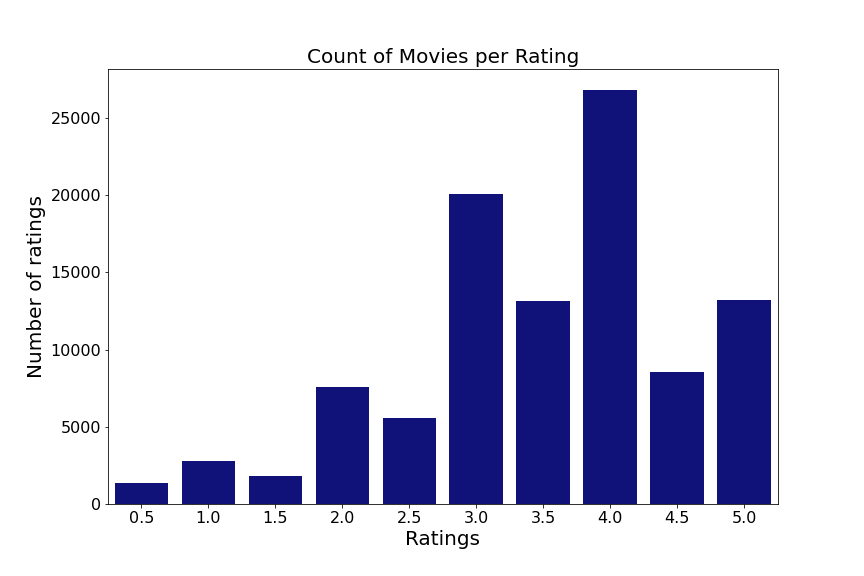
\includegraphics[width=0.99\textwidth]{count_rating.png}
  	\caption{Count of Movies per Rating}
  	\label{fig:count_ranking}
    \end{minipage}
    \hspace{0.01cm}
    \begin{minipage}[b]{0.49\linewidth}
        \centering
  	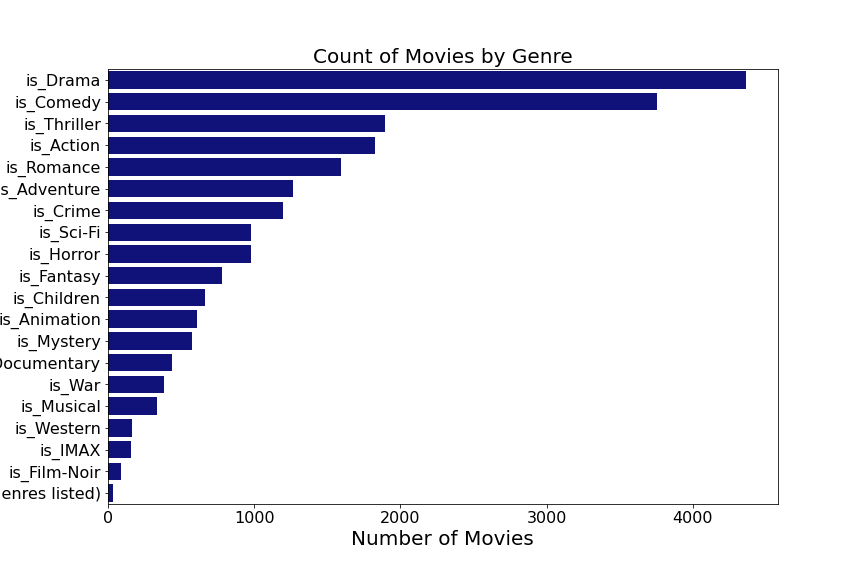
\includegraphics[width=0.99\textwidth]{count_genre.png}
  	\caption{Count of Movies per Genre}
  	\label{fig:count_genre}
    \end{minipage}
\end{figure}

The median user has rated about 70 films, whereas the user with the lowest number of watched films was 20 movies and the user with the highest number of rated films is 2,698. In Figure \ref{fig:ranking_ts}, the evolution of ratings over time is depicted. Despite some occasional spikes, the time series seems to have some seasonality. Furthermore, Figure \ref{fig:evolution_2} illustrates the trend in the number of movies rated 0 and 2, movies rated 3 to 10, etc. It is notable that users opt for films with fewer recommendations, probably because they are newly released films. However, most popular films gain more ratings over time which denotes the effect of richer get richer.

\begin{figure}[h!]
    \begin{minipage}[b]{0.49\linewidth}
        \centering
  	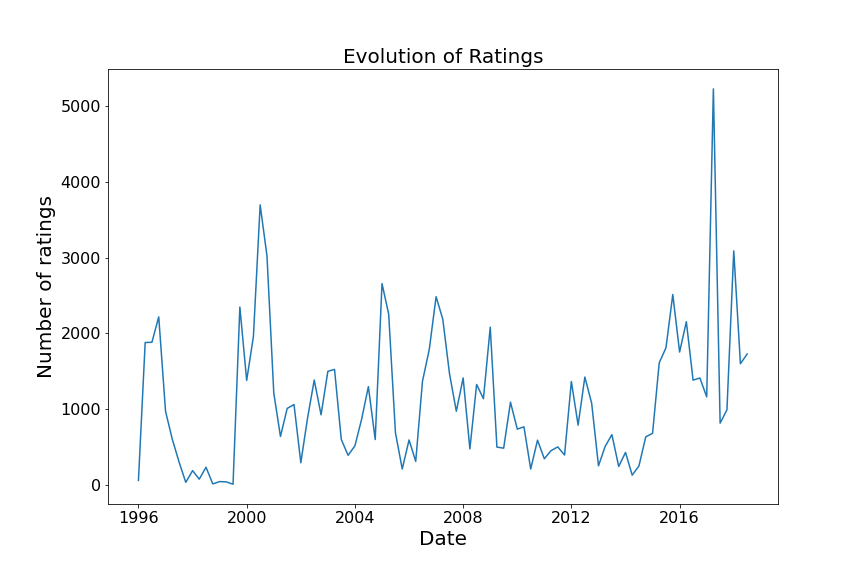
\includegraphics[width=0.99\textwidth]{ratings_evolution.png}
  	\caption{Evolution of ratings}
  	\label{fig:ranking_ts}
    \end{minipage}
    \hspace{0.01cm}
     \begin{minipage}[b]{0.49\linewidth}
         \centering
  	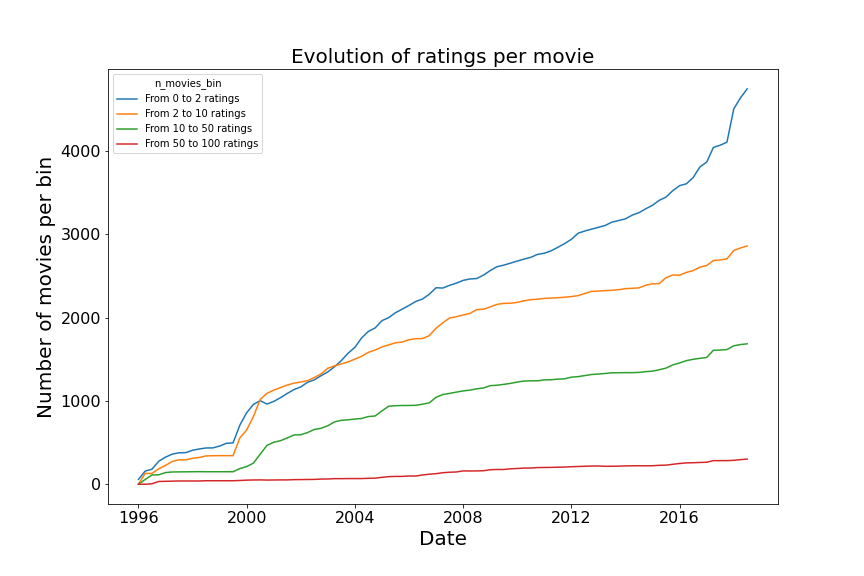
\includegraphics[width=0.99\textwidth]{ratings_evolution_2.png}
  	\caption{Evolution of ratings per movie}
  	\label{fig:evolution_2}
    \end{minipage}
\end{figure}

\section{Network analysis}

Using the MovieLens dataset, we create 4 different networks using the NetworkX package in python  The first, i.e. the user-movie network, serves as the foundation for the recommendation systems that we build. From this network, we also construct a user-to-user network - a symmetric unipartite network capturing the similarity between users. Similarly, we create a movie-to-movie network. Finally, we create another bipartite network that, instead of capturing relationships between users and specific movies, describes the "fan score" between a user and a genre of movie.

\subsection{User-to-movie bipartite network}

To create the user-to-movie bipartite network, we selected the unique User Ids as one set of nodes and the movie titles as another. Edges were then added if a user has seen a movie. Note that this is an undirected, unweighted graph, i.e. ratings are not considered.

Despite an incredibly sparse matrix, which is to be expected given the catalog of close to 10,000 movies, this results in a connected graph - i.e., there is only one component.

\begin{figure}[h!]
\centering
    \begin{minipage}[b]{0.49\linewidth}
         \centering
  	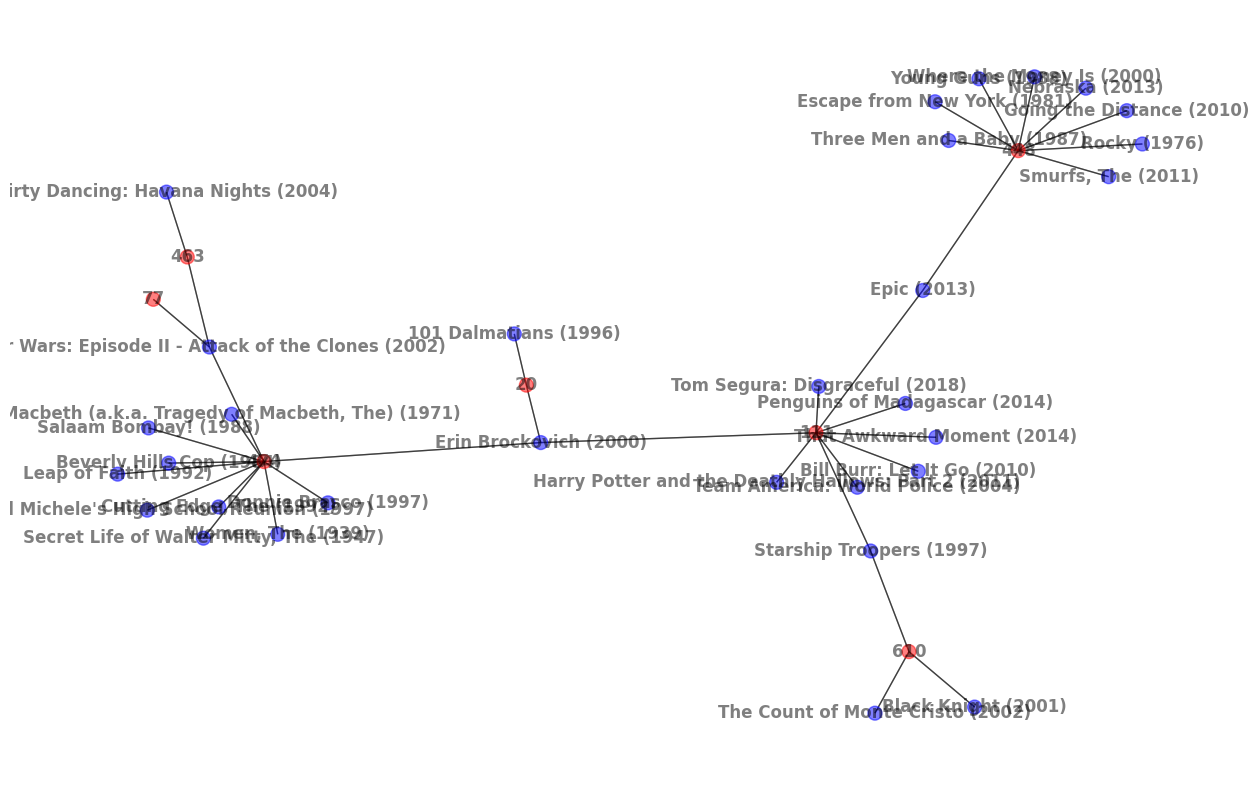
\includegraphics[width=0.99\textwidth]{sample_graph.png}
  	\caption{Subset of User to Movie Network}
  	\label{fig:count_ranking 2} 
    \end{minipage}
    \hspace{0.01cm}
    \begin{minipage}[b]{0.49\linewidth}
        \centering
  	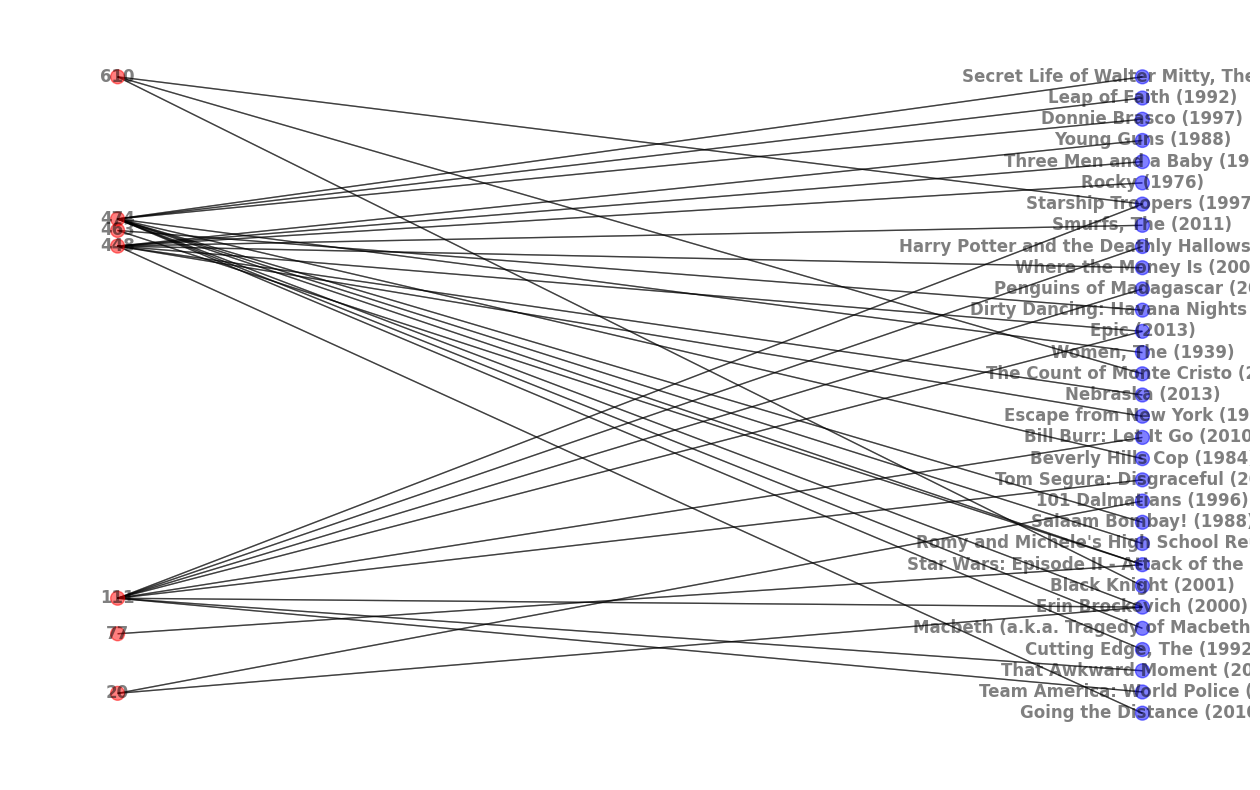
\includegraphics[width=0.99\textwidth]{bipartite.png}
  	\caption{BipartiteLayout}
  	\label{fig:ranking_ts 2}
    \end{minipage}
\end{figure}


To better understand the network, we calculated the centrality for for both users and movies (Figure \ref{fig:centrality}).
The degree centrality for users and movies are aligned with how many reviews they have. The centrality score for users is much higher than that for movies as there are generally many more reviews per user than there are per movie. 

However, this might not fully encapsulate all aspects of centrality. Therefore, we also calculated the betweenness and closeness centralities. Take, for example, The Avengers (2012). Regardless of how many reviews it may have, it is likely to be an important bridge (betweeness) between the Marvel movies. It is relationships like these that we are hoping to capture. However, there seems to be very little difference in the rankings of these centrality metrics as the top scores keep generally the same order. 

\begin{figure}[h!]
\centering
\caption{Network Centrality Measures and Comparative Metrics for Movies}
    \begin{tabular}{|c|c|c|c|}
        \hline
        \textbf{User Id} & \textbf{Degree Centrality} & \textbf{Betweeness Centrality} & \textbf{Closeness Centrality} \\ 
        \hline
        599 & 4.067 & 0.141 (1) & 0.406 (2) \\
        414 & 4.429 & 0.131 (2) & 0.413 (1) \\
        474 & 3.460 & 0.120 (3) & 0.395 (3) \\
        448 & 3.061 & 0.110 (4) & 0.388 (4) \\
        274 & 2.210 & - & 0.373 (5) \\
        610 & 2.136 & 0.060 (5) & 0.372 (6) \\
        68  & 2.067 & - & 0.371 (7) \\
        380 & 2.000 & 0.034 (10) & 0.370 (8) \\
        606 & 1.829 & 0.050 (6) & 0.367 (9) \\
        288 & 1.731 & - & 0.365 (10) \\
        \hline
    \end{tabular}

   \vspace{0.2cm} % Adjust the vertical space between tables as needed
    
    \begin{tabular}{|p{6cm}|r|r|r|}
        \hline
        \textbf{Movie Title} & \multicolumn{1}{p{2.5cm}|}{\textbf{Degree Centrality}} & \multicolumn{1}{p{3cm}|}{\textbf{Betweeness Centrality}} & \multicolumn{1}{p{3cm}|}{\textbf{Closeness Centrality}} \\
        \hline
        Forrest Gump (1994) & 0.0339 & 0.0064 & 0.4824 \\
        Pulp Fiction (1994) & 0.0316 & 0.0050 & 0.4650 \\
        Matrix, The (1999) & 0.0286 & 0.0048 & 0.4694 \\
        The Silence of the Lambs (1991) & 0.0287 & 0.0046 & 0.4624 \\
        Shawshank Redemption (1994) & 0.0326 & 0.0042 & - \\
        Star Wars: Episode IV (1977) & 0.0258 & 0.0041 & 0.4613 \\
        Jurassic Park (1993) & 0.0245 & - & - \\
        Braveheart (1995) & 0.0244 & - & - \\
        Terminator 2 (1991) & 0.0231 & - & - \\
        Schindler's List (1993) & 0.0226 & - & - \\
        \hline
    \end{tabular}
\label{fig:centrality}
\end{figure}

It is important to note already that the most highly centralized movies are all produced before 2000 (in fact, this extends far beyond just the top 10), despite most of the reviews coming after the 2020s. This is understandable as movies that have been around longer are more likely to have more reviews.

\subsection{User-to-User network}

To construct the user-to-user network, we calculated the similarity between all users as our edges.  We first pivoted the Ratings dataframe on the \textit{UserId},  making UserId the index, the Movies as the columns, and any user ratings inside. This is exactly the adjacency matrix for the User to Movie network that we created in the previous section; however, now with weighted edges based on ratings.

We used cosine similarity as our node embedding technique to map user vectors. Cosine similarity is a common similarity metrics because it ignores magnitude and focuses only on directions. For example, a harsh critic might rate an average movie a 2 but a more generous critic might consider average to be 3. This would not affect at all the cosine similarity. A similarity measure such as Euclidean distance would fail here because the more movies you add can only possibly add distance. Therefore people are punished for actually having seen more of the same films.

Because this is an incredibly sparse matrix, we only base similarity off the movies that users have in common. However, this could result in the case where two people are assigned similarities despite having watched very few of the same movies. For example, if two people who have wildly different preferences both watched one movie and both gave it 4 stars, these two people would be assigned a perfect similarity when, clearly, this should not be the case. To mitigate this, we only kept similarity scores for people that have rated 10 or more movies in common.

We calculate similarity scores using cosine similarities between users with each movie as a feature. Only movies where both users have given a rating are considered. Because ratings are all positive, all vectors will only be in the positive space. Therefore, cosine similarities are limited to only positive values as any two vectors cannot exceed more than a right angle. We constructed a similarity matrix using this framework which will henceforth in the paper be referred to as simply the User Network.

Again, these similarities can be conceived of as an adjacency matrix - this for a unipartite, weighted, bidirectional graph (i.e. the matrix is symmetric as the similarity from user a to user b is the same as user b to user a). From these graphs we made an unweighted graph by setting a threshold of 0.9 for the User Network and 0.5 for the Midrange-Adjusted User Network. These thresholds were chose as they both return similar numbers of edges (around 68,000). If the similarity score is greater than the threshold, an edge is created.

The degree distribution of this network can been seen in Figure \ref{fig:UN_degreeinfo} below.

\begin{figure}[h!]
    \begin{minipage}[b]{01\linewidth}
         \centering
  	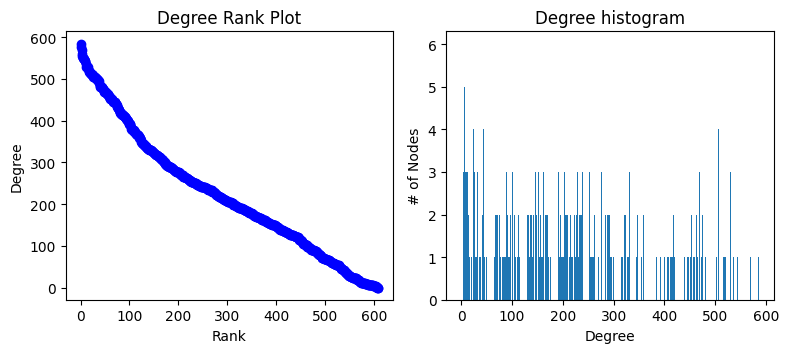
\includegraphics[width=0.9\textwidth]{UN_degreeinfo.png}
  	\caption{Degree Information for User Network}
  	\label{fig:UN_degreeinfo}
    \end{minipage}
\end{figure}

\subsection{Movie-to-Movie network}

A similar procedure can be done to obtain a similarity score matrix that will be considered as the adjacency matrix of the movie-to-movie network. Figure \ref{fig:MN_degreeinfo} describes the network distribution. 

\begin{figure}[h]
    \centering
  	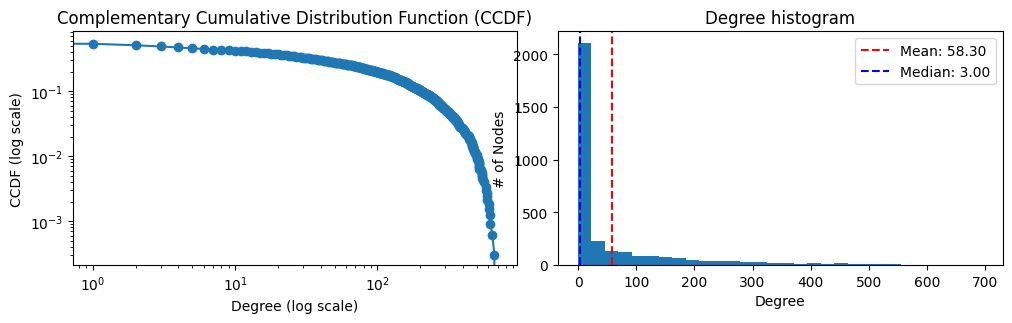
\includegraphics[width=0.8\textwidth]{movie2movie_analysis.png}
  	\caption{Degree Information for Movie Network}
  	\label{fig:MN_degreeinfo}
\end{figure}

In this section, community detection algorithms will be used to identify potential communities among the movies. The edges in the obtained undirected graph correspond to a similarity score between films that commonly users like have liked them. 

For community detection, we experimented with several options (Louvain, DC-SBM and greedy). Most of them take long to run for a network with 95,219 edges and 1,848 nodes, which is not a particularly large network. Greedy algorithm provided a good result in reasonable amount of time, it uses Clauset-Newman-Moore greedy modularity maximization to find the community partition with the largest modularity \cite{greedy}.

The modularity is defined as: 
\begin{equation}
Q = \frac{1}{2m} \sum_{ij} ( A_{ij} - \gamma \frac{k_i k_j}{2m}) \delta (c_i, c_j)
\end{equation}

where $m$ is the number of edges, $A$ is the adjacency matrix of G, $k_i$ is the (weighted) degree of $i$, $\gamma$ is the resolution parameter, and $\delta (c_i, c_j)$ is 1 if $i$ and $j$ are in the same community else 0. If resolution is less than 1, modularity favours larger communities. Greater than 1 favours smaller communities.

The greedy algorithm detects 10 communities, with a modularity of 0.18163. Only 5 communities have more than 10 movies (or nodes) in them. In Figure \ref{fig:comm_detection}, the different communities in the graph can be observed.

\begin{figure}[h!]
    \centering
  	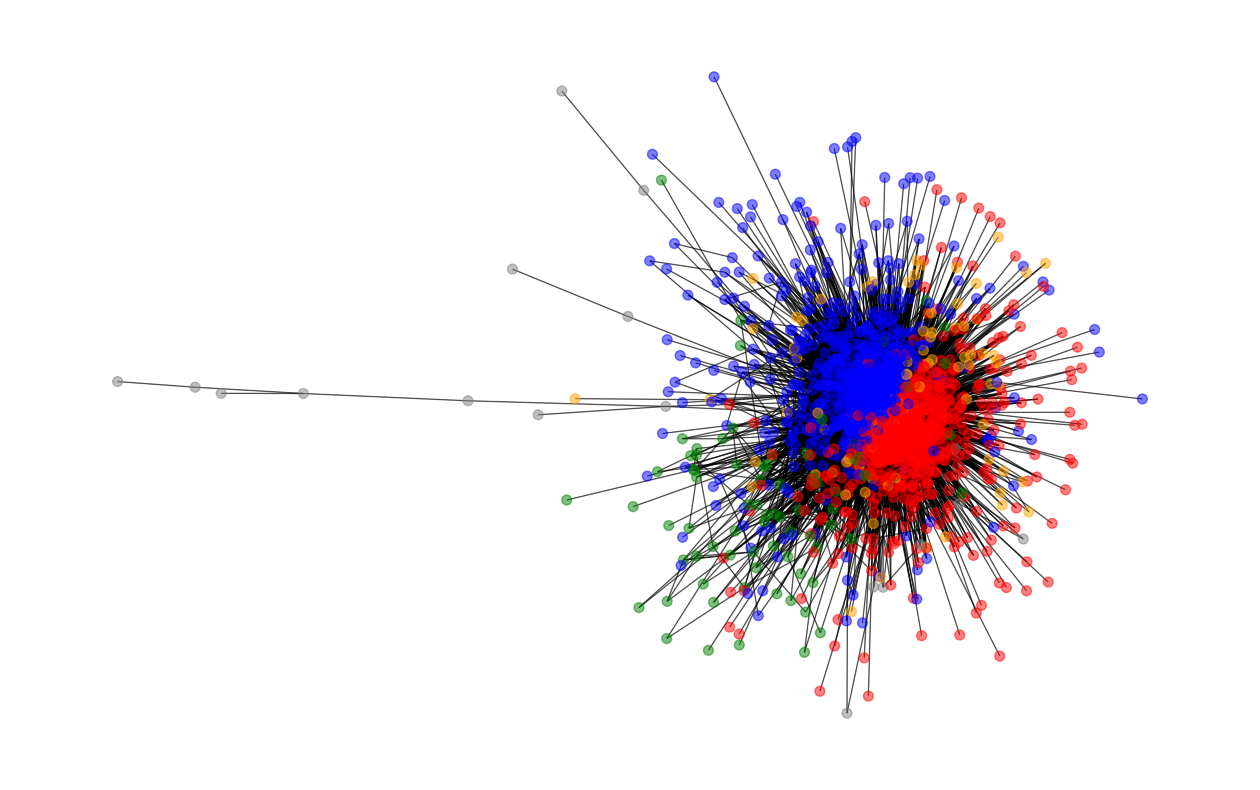
\includegraphics[width=0.8\textwidth]{community_detection.png}
  	\caption{Movie Network communities}
  	\label{fig:comm_detection}
\end{figure}


\subsection{User-to-Genre network}

Many recommendation systems, including Random Walks and Collaborative Filtering which we will discuss later, only take into account user and item interactions. The content of the films is irrelevant and no relationship between the items is captured beyond what was described in the matrices above. Clearly, if we were able to capture these relationships, we could then build much stronger recommendations. One simple ubiquitous covariate is the genre of the film. It wouldn't feel quite right to sit down for family movie night and be recommended The Shining because you watched The Lion King last week - despite both movies probably having somewhat similar cosine similarity as both movies are generally well regarded. Item-to-item recommendations should consistently stay within the same category and, often, user-recommendations are filtered by said categories.

Therefore, we took a network approach to deepen our understanding between users and genres. Our goal is to quantitatively capture relationships between users and genres that could, in principle, be used to provide better recommendations. We a

In order to do this, movies are classified into their respective genres. Movies with no listed genres were dropped. Subsequently, we computed both the overall average rating for each user and their genre-specific average ratings. Additionally, we tallied the total number of reviews submitted by users, alongside a genre-wise review count, to capture a detailed view of user engagement and preferences. Finally, we used the following formula to determine whether or not someone was a fan of a particular genre. 

\[
\text{F}_{gi}= \text{tanh}\left(\frac{P_{gi} R_{gi}\ln(C_{gi})}{3}\right)
\]

$P_g$ is the percentage of user reviews within genre $g$. Naturally, if a larger percentage of a person's movies belong to a single genre, this should be rewarded. Similarly, $R_g$ represents the average review for a user within a genre. The higher the reviews, the greater the score. Finally, we wanted to factor in the number of films within the genre watched. While this should be somewhat accounted for in $P_g$, this may be helpful for identifying super fans or "influencers". This is reward logarithmically and we divide by 3 as a scaling constant.
This is then passed through tanh to give us fan scores between 0 and 1 (as this score can never be negative unless we adjust with midrange which then could capture a possible "hater score").

Then we arbitrarily chose 0.8 as the threshold. For users with over a 0.8, they were considered a fan.  The number of fans per genre and a visual representation of the network can be seen in Figures 4.7  below.

\begin{figure}[h!]
\label{fig:fanspergenre}
    \begin{minipage}[b]{0.49\linewidth}
         \centering
  	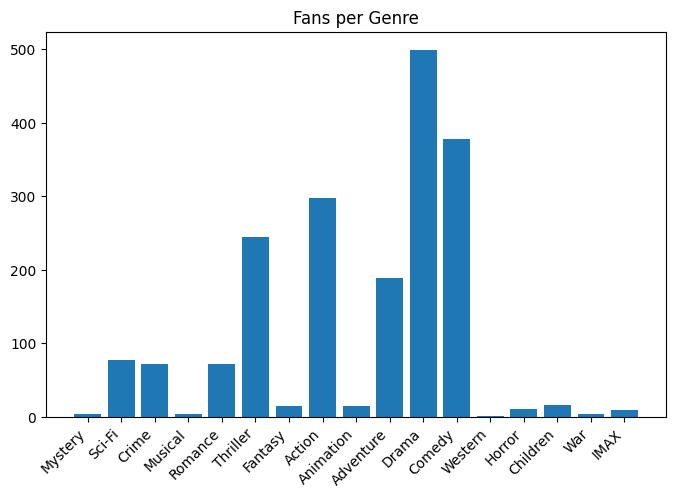
\includegraphics[width=0.99\textwidth]{fans_per_genre.png}
	 \caption{Fans per Genre}
    \end{minipage}
    \hspace{0.01 cm}
    \begin{minipage}[b]{0.49\linewidth}
         \centering
  	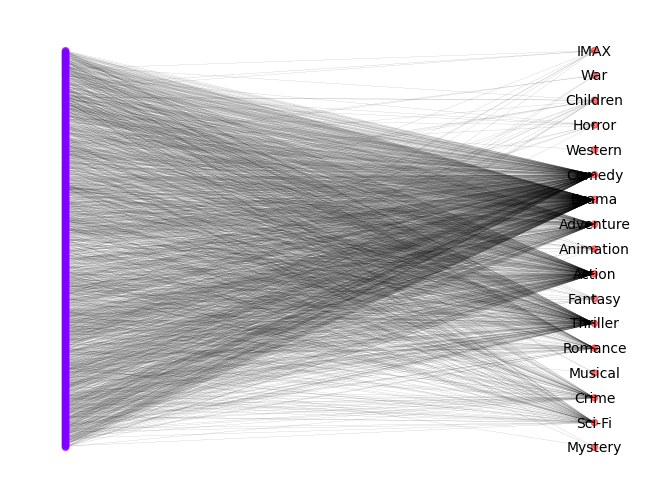
\includegraphics[width=0.99\textwidth]{genre_bipartite.png}
  	\caption{\\Users - Genre Bipartite Graph}
\label{fig:genre_bipartite}
    \end{minipage}
\end{figure}

Once again, we can create an unweighted bipartite adjacency matrix from this with the users as one set of nodes and the movies as the other (visualized in Figure \ref{fig:genre_bipartite}).

Here, the degree represents how the number of genres for which that user is considered a fan. With the degree histogram, we see a strong fit of a binomial distribution with $n = 19$ (the number of genres) and $p = \frac{4.5}{19}$

\begin{figure}[h!]
    \begin{minipage}[b]{1\linewidth}
         \centering
  	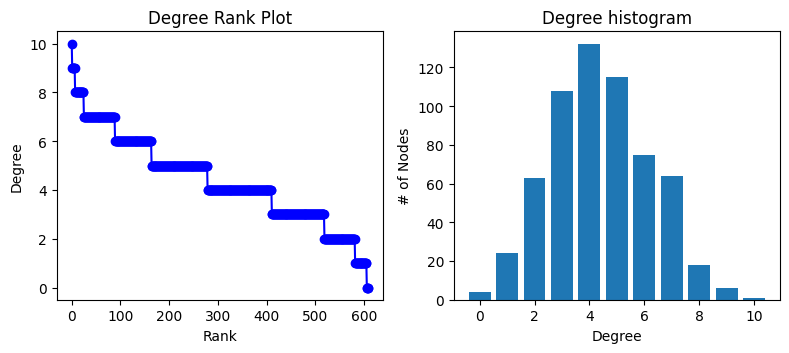
\includegraphics[width=0.99\textwidth]{genre_degree1.png}
  	\label{fig:fanspergenre}
	 \caption{User Degrees}
    \end{minipage}
    \vspace{0.1cm}
    \begin{minipage}[b]{1\linewidth}
         \centering
  	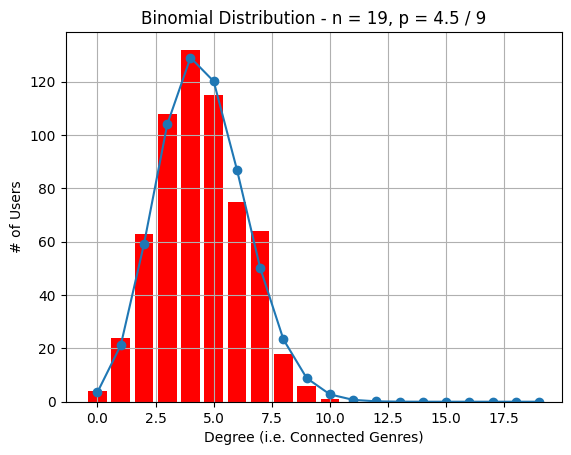
\includegraphics[width=0.5\textwidth]{binomialfit.png}
  	\label{fig:fanspergenre}
    \end{minipage}
\end{figure}

However, looking at Figure 4.7, we see an issue. It appears that we are just measuring how many movies there are per genre. Our formula, while it could be effective for large relatively balanced sets, fails in this context. Therefore, we attempt to create a definition of "fan" that is more accounts for movie imbalances.

\[
F_{gi}^* = \left(\frac{R_{gi} - R_i}{R_g}\right)\mathbbm{1}{\{C_g > 10\}}
\]

This simplified version finds the difference between a user's score per genre with the average rating per genre and normalizes it by the average rating of that user. The threshold for being a fan here was set to 0.5. The results can be seen in the Figures below:

\begin{figure}[h!]
    \begin{minipage}[b]{0.5\linewidth}
         \centering
  	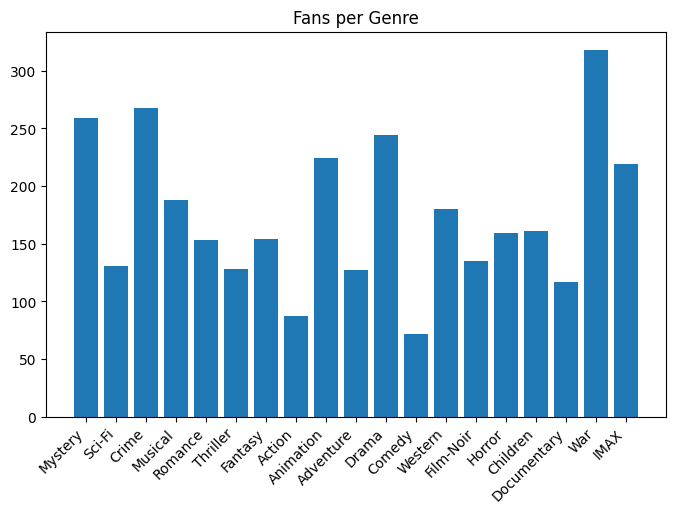
\includegraphics[width=0.99\textwidth]{fansgenre1.png}
  	\label{fig:fanspergenre}
	 \caption{New Fans per Genre}
    \end{minipage} 
    \hspace{0.1cm}
    \begin{minipage}[b]{0.5\linewidth}
         \centering
  	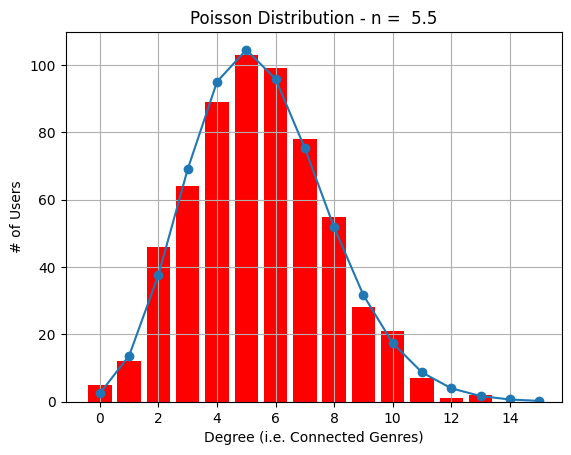
\includegraphics[width=0.99\textwidth]{poissondegree.png}
  	\label{fig:fanspergenre}
	 \caption{Poisson fit with $n = 5.5$}
    \end{minipage} 
\end{figure}

The distribution of fans across genres is now much more even and the degree distribution among fans aligns closely a Poisson with mean 5.5.

\section{Random Walk Recommendation Systems}

In this section, we explore recommendation systems that directly leverage the network structure of the data. Specifically, we focus on the Probabilistic Spreading (ProbS) and Heat Spreading (HeatS) algorithms, which employ a random walk process within a binary user-item bipartite network to provide a ranking to movies that a user has not seen.

For a given user \textit{i} , the ProbS algorithm initialises by giving a unit amount of resource to all items that they are connected to. The algorithm then employs a two-step random walk process to redistribute these resources, aiming to accentuate items preferred by users with similar tastes.

In the first step, each item's allocated resource is evenly distributed among users connected to it. This step effectively maps out the extent of shared interests between users based on the items they are associated with. Subsequently, the second step redistributes the resources accumulated by each user back to the items they are connected to, but now the distribution is equal among all such items. Through this reciprocal resource exchange, the algorithm iteratively refines the weight or importance of each item based on the density and depth of shared user preferences. Finally, the scores of items already connected with user \textit{i} are set to zero so as to not recommend items already connected with the user. A graphical representation of this process is shown in Figure \ref{subfig:prob_s}.

HeatS works in a very similar way to ProbS except a nodes score in the first and second steps are calculate as a simple average of the nodes it is connected to. A  graphical representation of this process is shown in Figure \ref{subfig:heat_s}.

\begin{figure}[!ht]
\centering
\begin{subfigure}[b]{0.45\textwidth}
    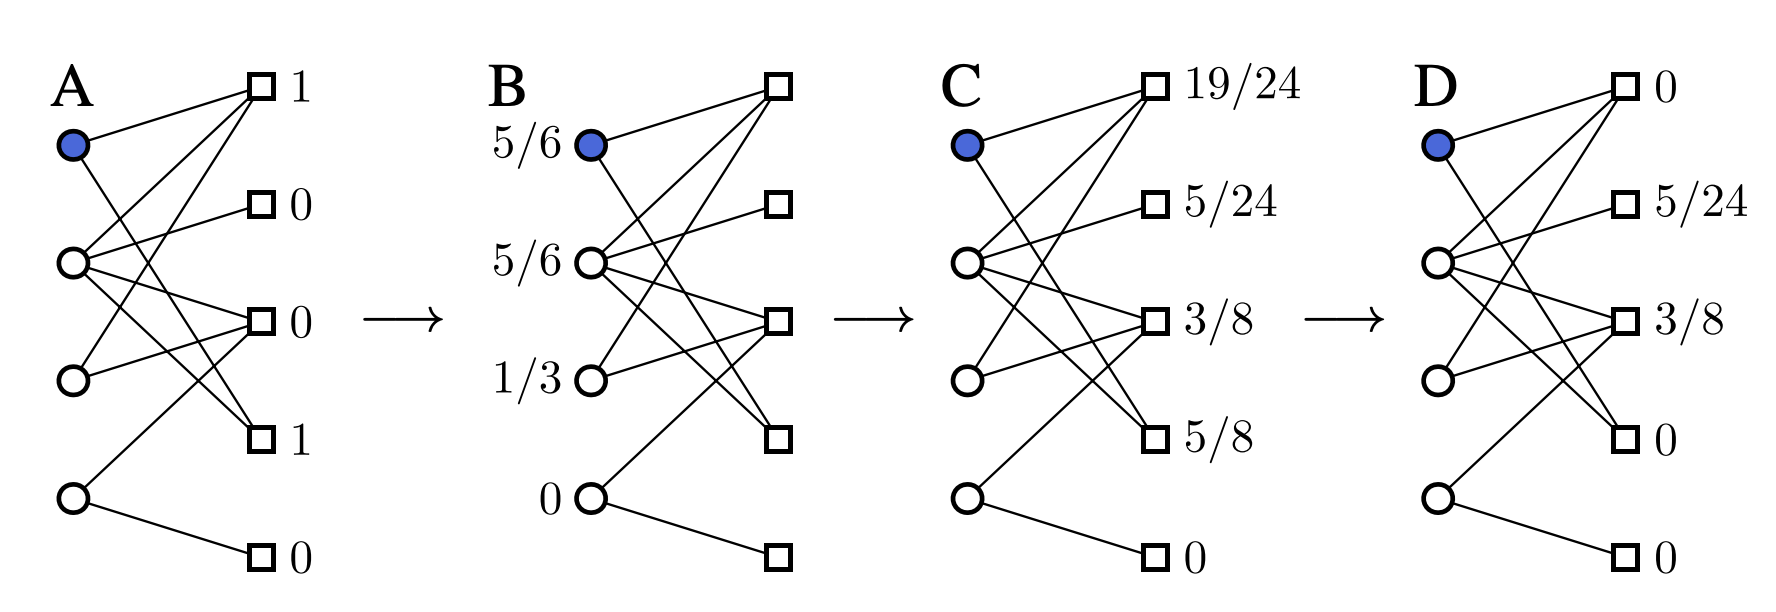
\includegraphics[width=\textwidth]{Prob S algorithm}
    \caption{ProbS Algorithm}
    \label{subfig:prob_s}
\end{subfigure}
\hfill % This adds space between the two subfigures
\begin{subfigure}[b]{0.45\textwidth}
    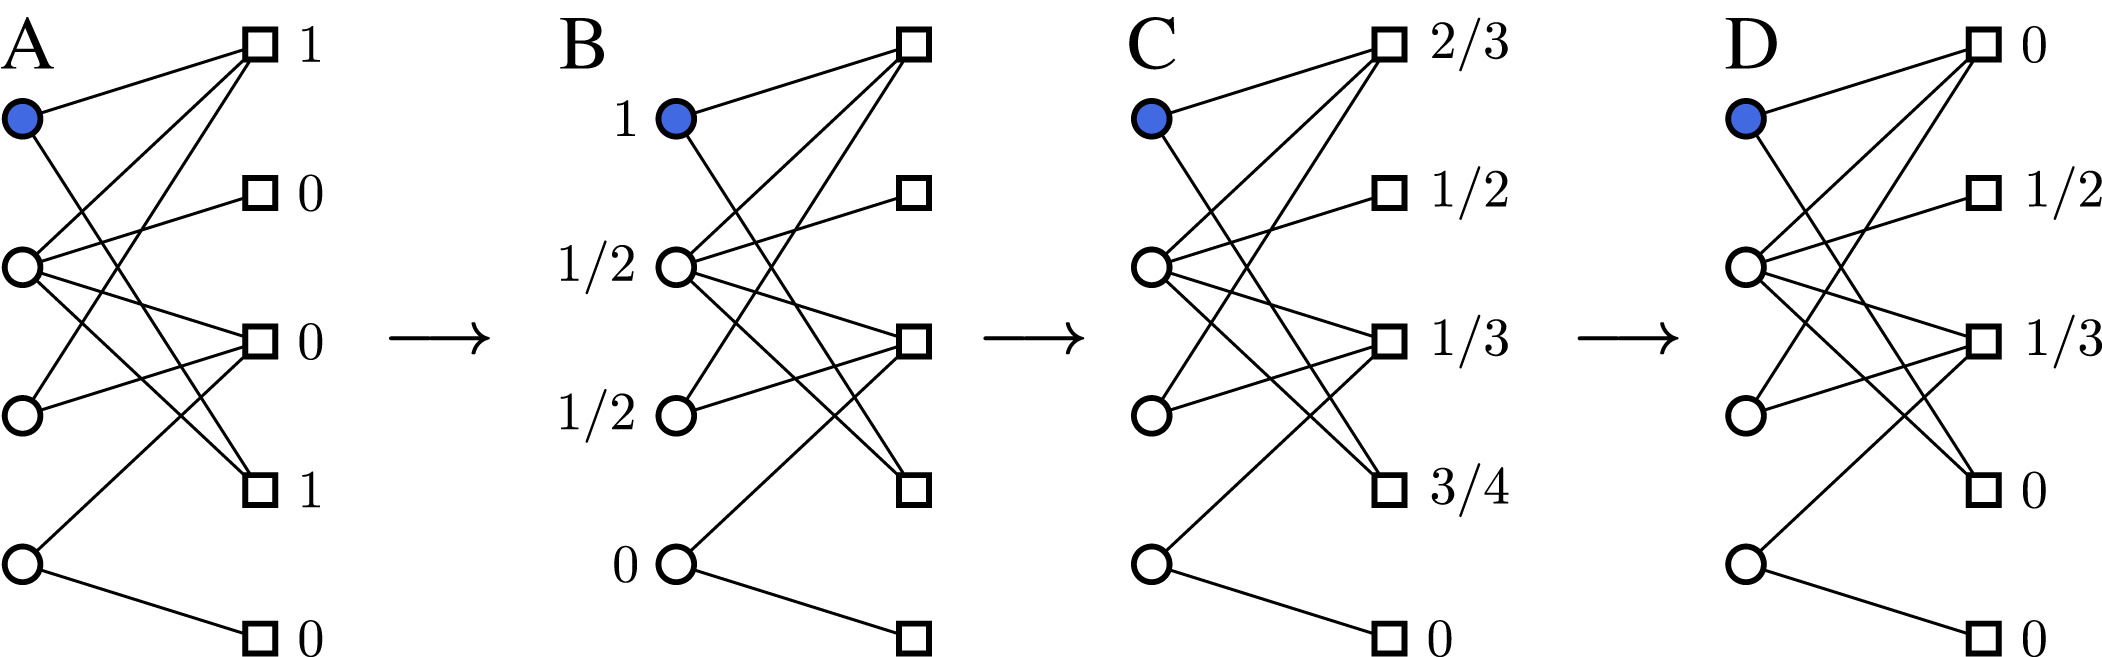
\includegraphics[width=\textwidth]{Heat S.jpg}
    \caption{HeatS Algorithm}
    \label{subfig:heat_s}
\end{subfigure}
\caption{Illustrations of the Probabilistic Spreading (ProbS) and Heat Spreading (HeatS) algorithms. In both diagrams, circles and squares represent users and items, respectively. The color-marked circle signifies the target user for whom the recommendations are being computed. Figures adapted from \cite{prob_s}.}
\label{fig:algorithms}
\end{figure}

Although the distinction between the two algorithms is subtle, there is a stark difference between the recommendations they produce. The ProbS method exhibits a stronger preference for popular items as the process is cumulative; therefore, an item enhances its likelihood of achieving a high score by accumulating numerous links. In contrast, the HeatS approach tends to favour less popular items. This preference is due to the averaging nature of the HeatS algorithm, where an item can increase its potential for a high score by having a limited number of links to users who possess a significant amount of resource value. This distinction between the two methods highlights their unique approaches to leveraging network dynamics, where ProbS capitalizes on the popularity and widespread connectivity of items, whereas HeatS leverages the principle of scarcity and targeted endorsements from highly resourced users.

As an extension of these algorithm, we also experiment with initialising weights proportional to the rating a user gave each movie. By doing so, we hope to provide prioritise movies that the user enjoyed more, potentially leading to more tailored recommendations. 


\subsection{Temporal Analysis}

To gain deeper insights into the long-term effects of these recommendation algorithms, we examine the evolving dynamics of the network with iterative applications of the algorithm. In each cycle, we posit that the user selects and watches the top-recommended movie, subsequently leading to an update of the binary bipartite network to reflect this new user-item interaction. The recommendation algorithm is then reapplied, taking into account the updated state of the network. This process is repeated, allowing us to observe how the network—and thus the recommendations—might evolve over time with continuous user engagement.

Figure \ref{fig:temporal prob S} shows the recommendation counts after 1,  10 and 100 iterations of the binary ProbS algorithm, and the effect this has on the degree of each user.  The recommendation counts clearly illustrates a power-law distribution, indicating a strong preference by the algorithm for particular items. As a result, certain movies become highly connected, reaching a saturation point where nearly all users have watched with them. This saturation compels the algorithm to diversify its recommendations, thereby incrementally expanding the range of movies suggested to users. 


\begin{figure}[!ht]
\centering

% First row with three figures
\begin{subfigure}[b]{0.32\textwidth}
    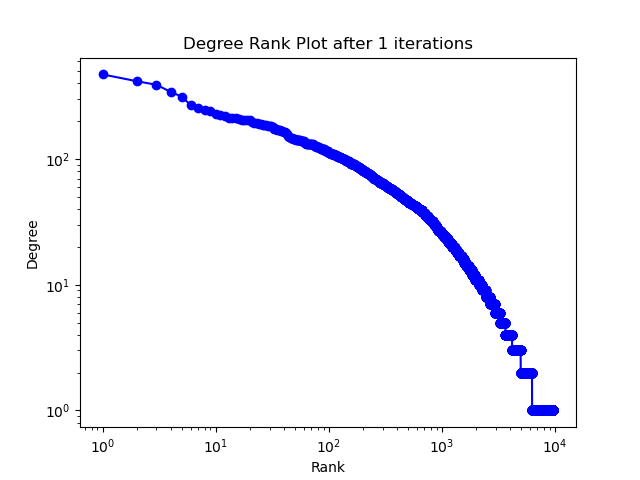
\includegraphics[width=\textwidth]{Prob S movie rank plot - 1 iterations.png}
\end{subfigure}
\hfill
\begin{subfigure}[b]{0.32\textwidth}
    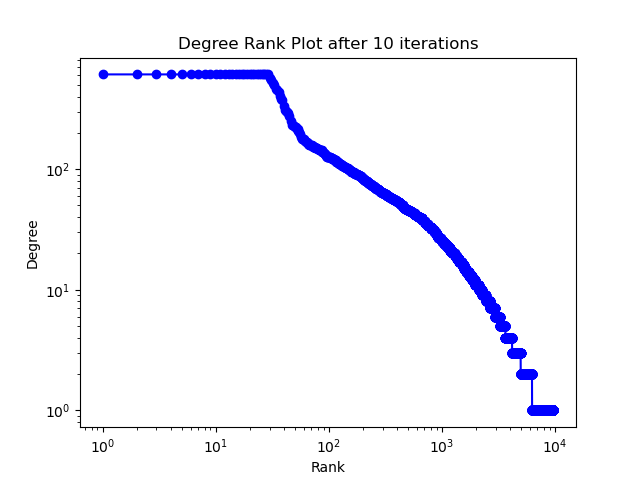
\includegraphics[width=\textwidth]{Prob S movie rank plot - 10 iterations.png}
\end{subfigure}
\hfill
\begin{subfigure}[b]{0.32\textwidth}
    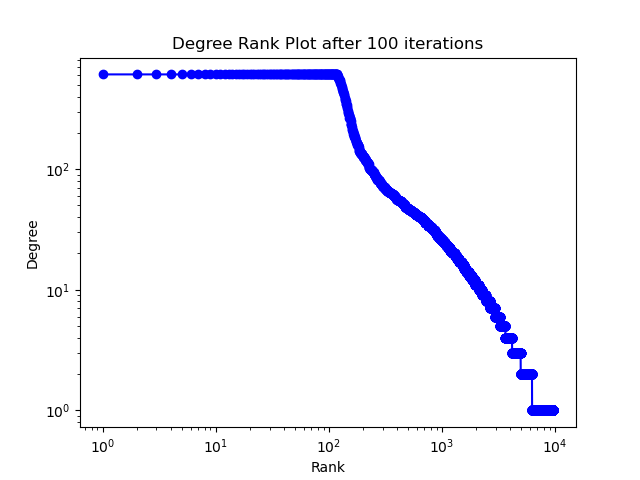
\includegraphics[width=\textwidth]{Prob S movie rank plot - 100 iterations.png}
\end{subfigure}

\vspace{1em} % Add some vertical spacing between the rows

% Second row with three figures
\begin{subfigure}[b]{0.32\textwidth}
    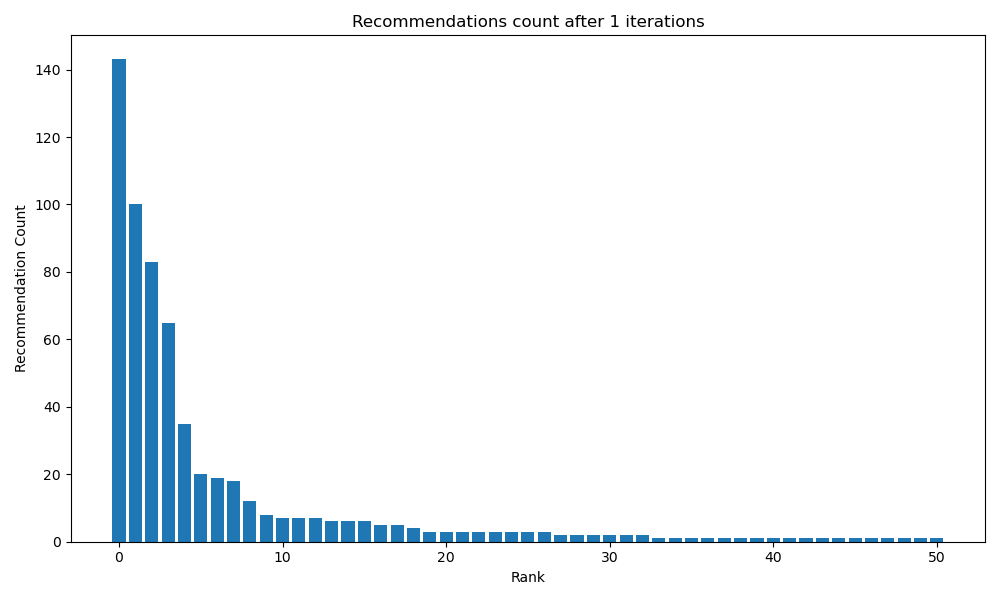
\includegraphics[width=\textwidth]{Prob S movie recommendations - 1 iterations.png}
\end{subfigure}
\hfill
\begin{subfigure}[b]{0.32\textwidth}
    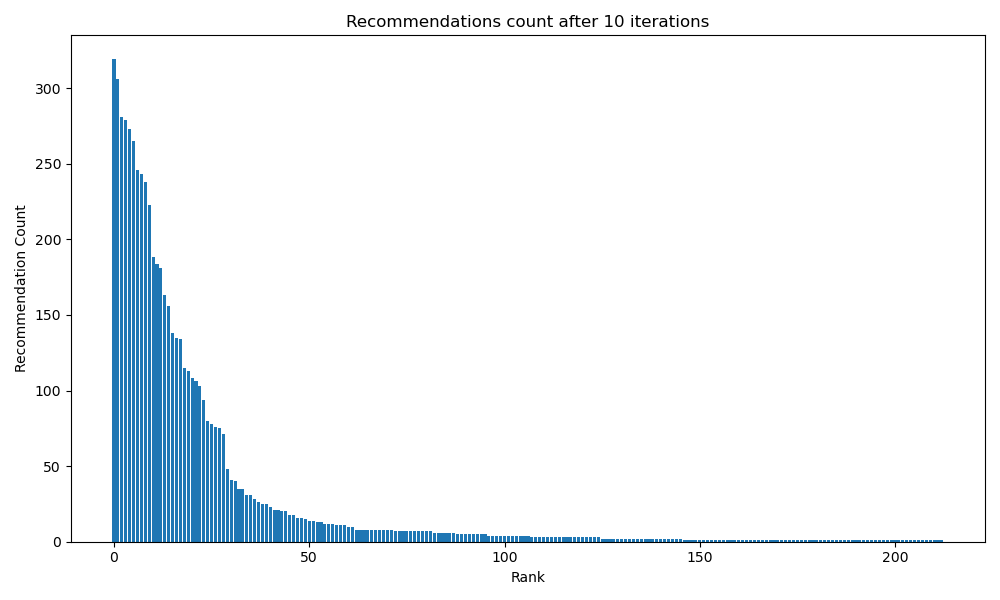
\includegraphics[width=\textwidth]{Prob S movie recommendations - 10 iterations.png}
\end{subfigure}
\hfill
\begin{subfigure}[b]{0.32\textwidth}
    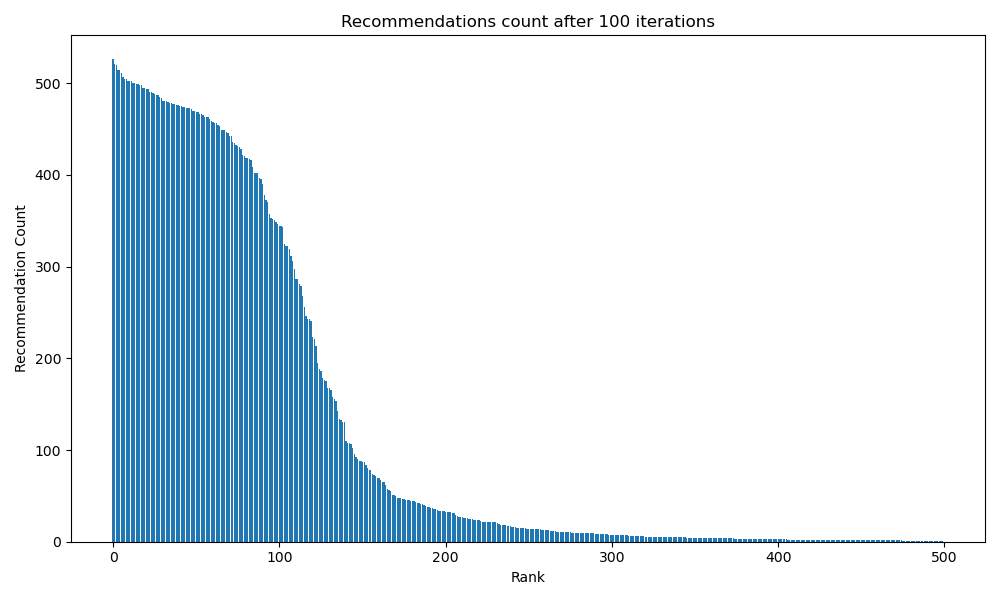
\includegraphics[width=\textwidth]{Prob S movie recommendations - 100 iterations.png}
\end{subfigure}

\caption{ProbS - Recommendation Dynamics}
\label{fig:temporal prob S}

\end{figure}

Figure \ref{fig:temporal heat S} shows the temporal analysis of the binary HeatS algorithm. Unlike ProbS, HeatS distributes its recommendations more evenly among items, as evidenced by the flatter distribution of recommendation counts over iterations. Items less connected in the user-item bipartite network are given relatively higher visibility, shown by the degree of lesser connected movies increasing while that of more connected films stays relatively unchanged. This prevents the dominance of a few movies, giving users recommendations from a broader array of content.

\begin{figure}[!ht]
\centering

% First row with three figures
\begin{subfigure}[b]{0.32\textwidth}
    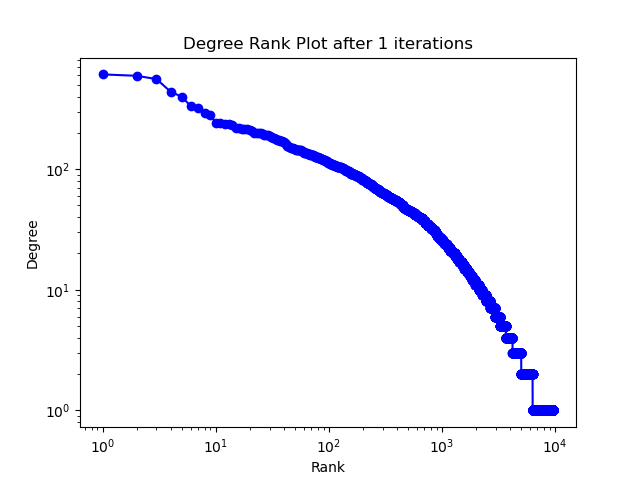
\includegraphics[width=\textwidth]{Heat S movie rank plot - 1 iterations.png}
\end{subfigure}
\hfill
\begin{subfigure}[b]{0.32\textwidth}
    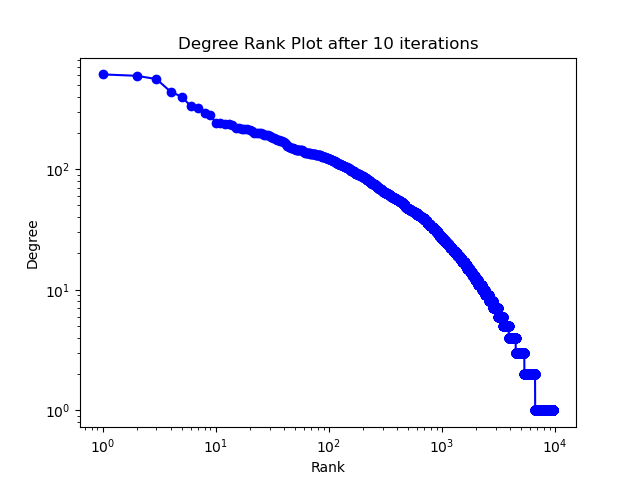
\includegraphics[width=\textwidth]{Heat S movie rank plot - 10 iterations.png}
\end{subfigure}
\hfill
\begin{subfigure}[b]{0.32\textwidth}
    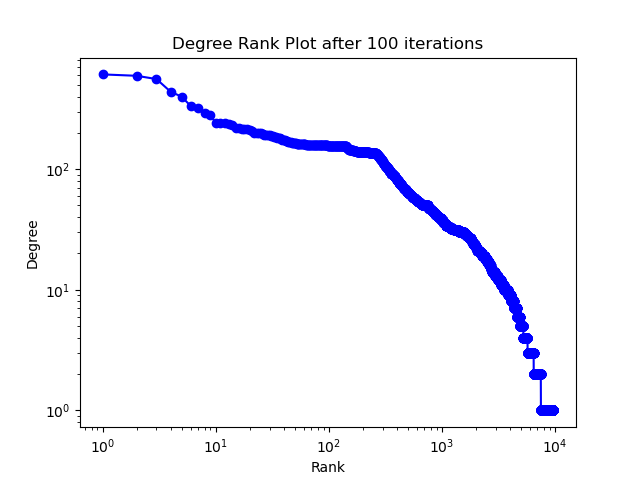
\includegraphics[width=\textwidth]{Heat S movie rank plot - 100 iterations.png}
\end{subfigure}

\vspace{1em} % Add some vertical spacing between the rows

% Second row with three figures
\begin{subfigure}[b]{0.32\textwidth}
    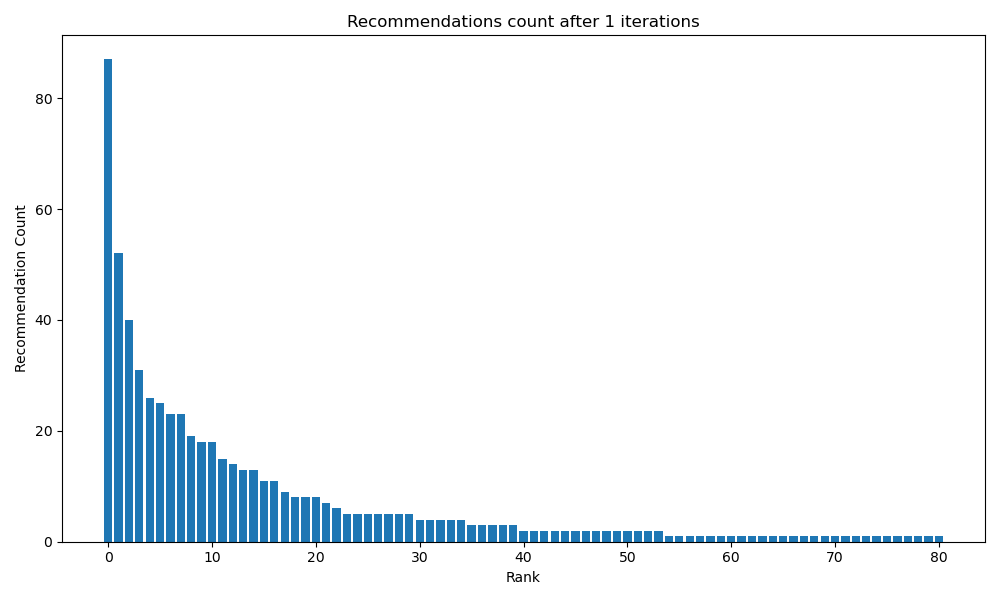
\includegraphics[width=\textwidth]{Heat S movie recommendations - 1 iterations.png}
\end{subfigure}
\hfill
\begin{subfigure}[b]{0.32\textwidth}
    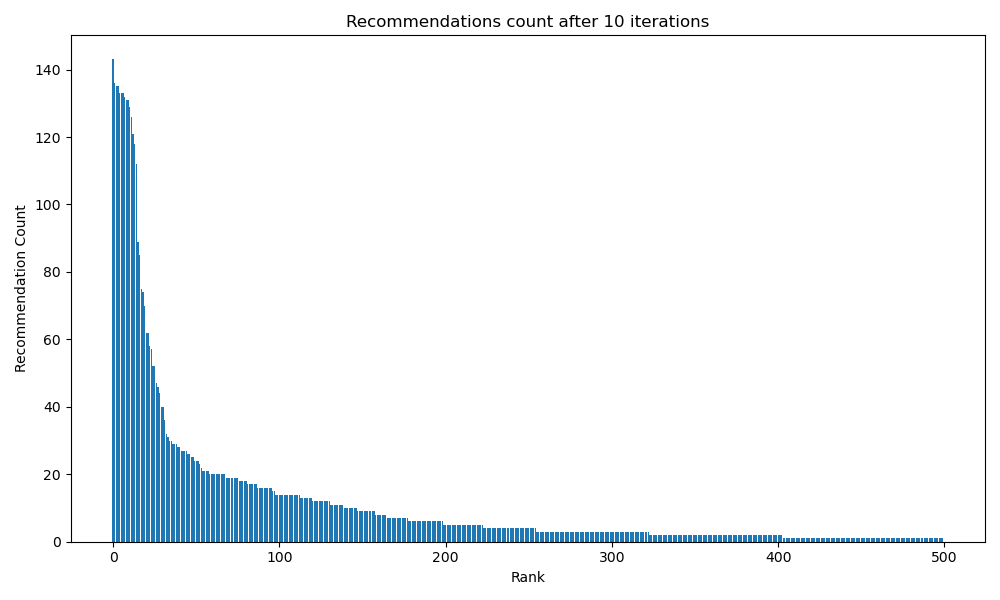
\includegraphics[width=\textwidth]{Heat S movie recommendations - 10 iterations.png}
\end{subfigure}
\hfill
\begin{subfigure}[b]{0.32\textwidth}
    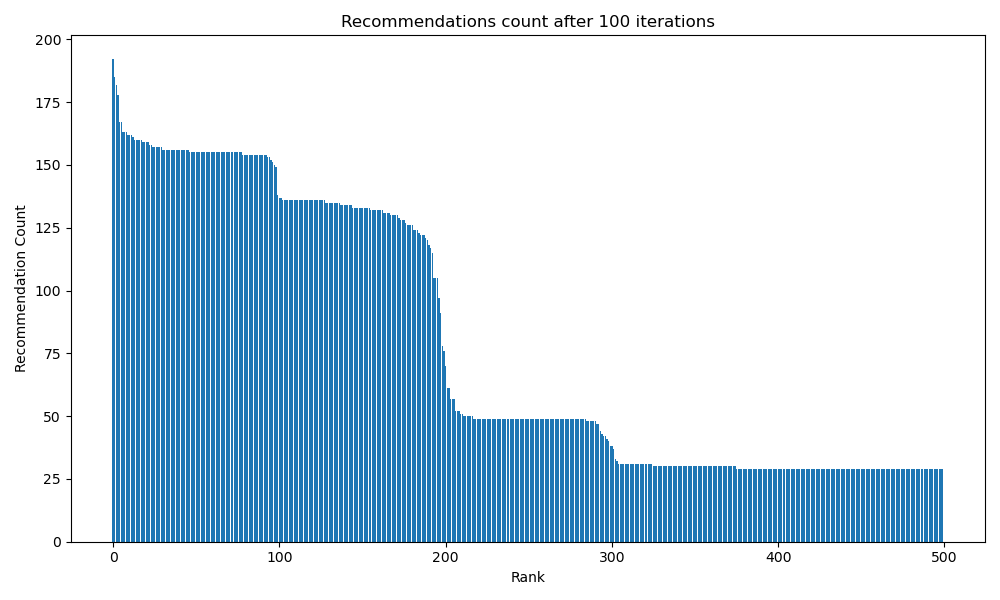
\includegraphics[width=\textwidth]{Heat S movie recommendations - 100 iterations.png}
\end{subfigure}

\caption{HeatS - Recommendation Dynamics}
\label{fig:temporal heat S}

\end{figure}



\subsection{Validation}

In order to evaluate the effectiveness of these recommender system, we perform a train-test split by randomly removing 20\% of each users ratings and subsequently calculate the Area Under the Curve (AUC) and average precision (i.e. percentage of recommendations that were actually liked by the user). The AUC is a performance metric used to evaluate the quality of binary classification models, which seemed a natural way to assess the performance of these algorithms since we can easily normalise the recommendation score given to be between 0 and 1. It represents tradeoff between the true and false positive rates at various threshold settings. The AUC ranges from 0 to 1, where a model with an AUC of 1 perfectly distinguishes between the two classes, and an AUC of 0.5 indicates no discriminative power, equivalent to random guessing. For the evaluation, a movie in the test set is deemed "liked" by a user if its rating exceeds the user's average rating across all movies in the training set, and thus we classify it as a good movie for the algorithm to recommend. To benchmark the results, we also calculate the average precision and AUC for a recommender system simply based on the average rating for each movie.

\begin{figure}[!ht]
    \centering  % Centers the table
    \begin{tabular}{|p{6cm}|r|r|}
        \hline
        \textbf{Model} & \multicolumn{1}{p{4cm}|}{\textbf{AUC}} & \multicolumn{1}{p{4cm}|}{\textbf{Average Precision}}  \\
        \hline
        Using Average Rating & 0.67 & 0.67 \\
        Prob S - uniform weight & 0.57 & 0.62 \\
        Prob S - using ratings & 0.59 & 0.62 \\
        Heat S - uniform weight & 0.51 & 0.54 \\
        Heat S - using ratings & 0.54 & 0.57 \\
        \hline
    \end{tabular}
    \caption{ProbS - Model performance} % Add your caption
    \label{fig:prob s performance} % Label your figure for reference
\end{figure}

As shown in Figure \ref{fig:prob s performance}, both the ProbS and HeatS models perform worse than the recommendations from using a movies average rating, with the incorporations of ratings only resulting in a small improvement. Furthermore, HeatS only performs slightly better than random. This underperformance could be due to data sparsity and the "cold-start problem", where the algorithms struggles to make accurate predictions because of insufficient user-item interaction data. In contrast, average ratings don't rely on user interaction and can recommend popular items effectively.

This said, the poor performance of the random walk models in terms of AUC does not necessarily mean that they are of no use. One key limitation is that our assessment is based solely on the movies held out in test that a user has already watched. These models might excel at suggesting new and diverse content that aligns with user preferences, yet this aspect remains unmeasured in this setting. This is likely to be particularly true of HeatS, which offers a more diverse array of suggests than ProbS or HeatS, which will often recommend items a user is already aware of.

\section{Collaborative Filtering}
For comparison, we implemented a basic user-based Collaborative Filtering system. Using the user-to-user similarity network and user-to-movie reviews, we are able to calculate predicted scores using the following formula:

\[
\hat{R_j} = \frac{\sum_{i=1}^n S_{ij}R_i}{\sum_{i=1}^n S_{ij}}
\]

$R_j$ is the predicted score for user j and $S_{ij}$ is the similarity score between user i and user j. Essentially, we are taking an average of all other reviews weighting by similarity score.

One issue we identified is that some movies were consistently getting predicted at 5.0 as a result of them only having one or two reviews, each of which was a perfect score. To combat this, we only apply this formula to movies that user j hasn't seen with at least 5 people in common (at least 5 similarities).

To pick a recommendation for a user, we cycle through all movies that the user j hasn't seen and calculate predicted scores. We then select recommendations based off of highest predicted ratings.

\begin{figure}[h!]
    \begin{minipage}[b]{01\linewidth}
         \centering
  	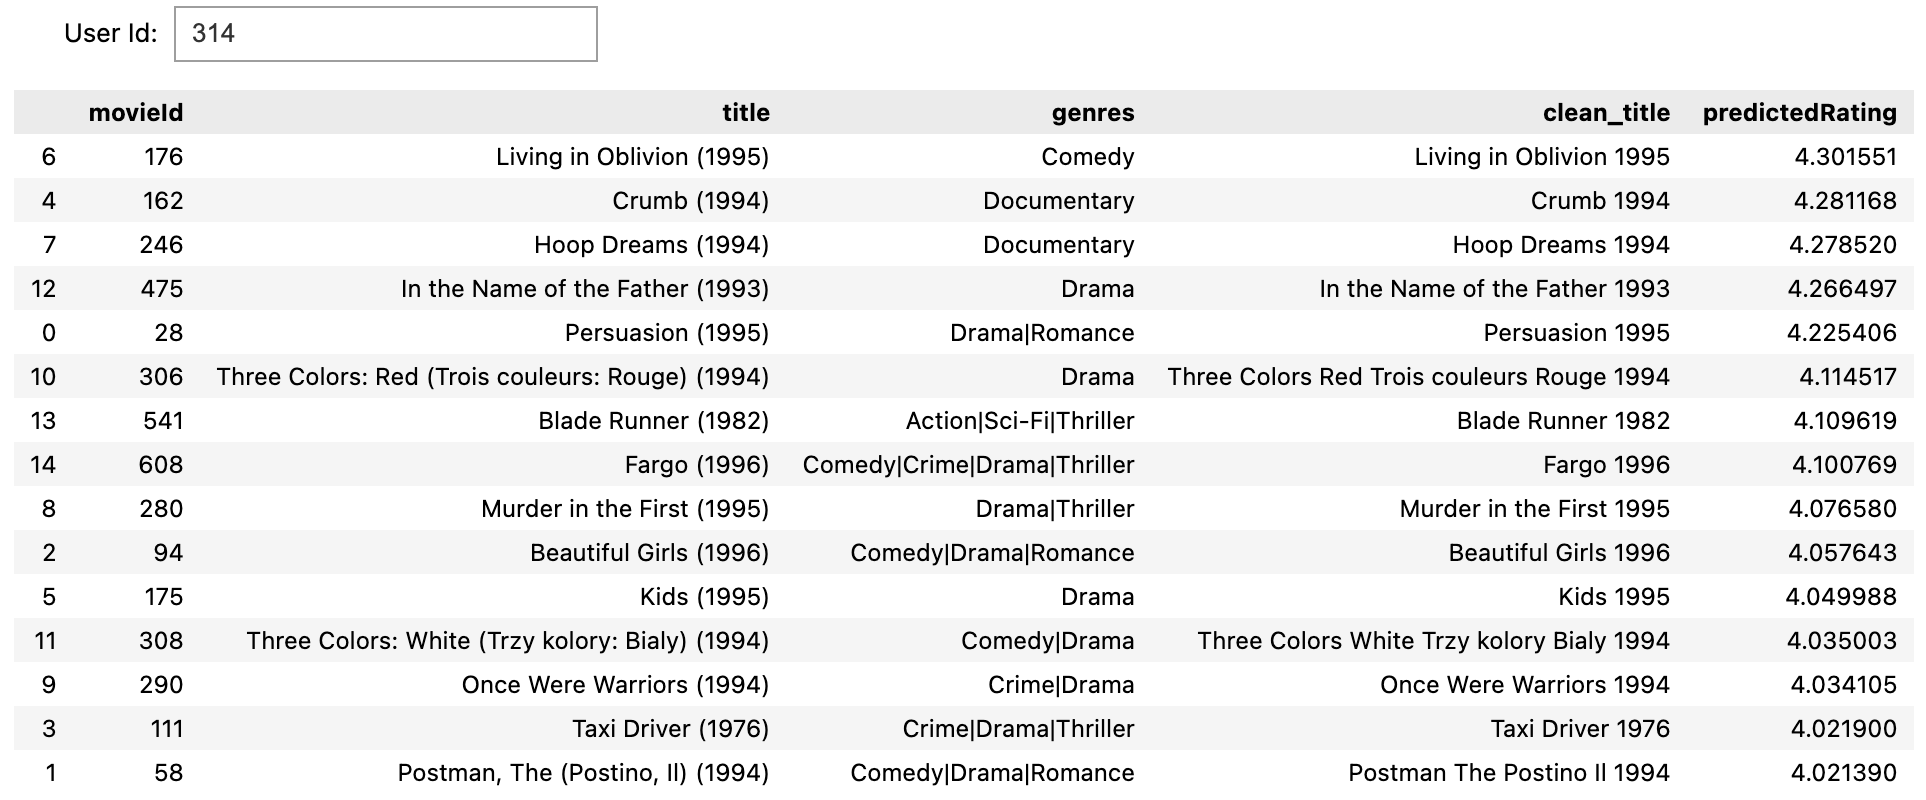
\includegraphics[width=0.9\textwidth]{314_recs}
  	\caption{Recomendations for User 314}
  	\label{fig:UN_degreeinfo}
    \end{minipage}
\end{figure}

After running this for every single user, we see a pattern for the top reviews recommend. Figure \ref{fig:top_recs_cf} shows that top 10 top-recommended movies. We see the cold start problem. All top recommended movies are movies that are generally highly rated and with a lot of reviews. All top 10 movies were released before 2000 despite this being not at all representative of the total population of movies.

\begin{figure}[h!]
    \begin{minipage}[b]{01\linewidth}
         \centering
  	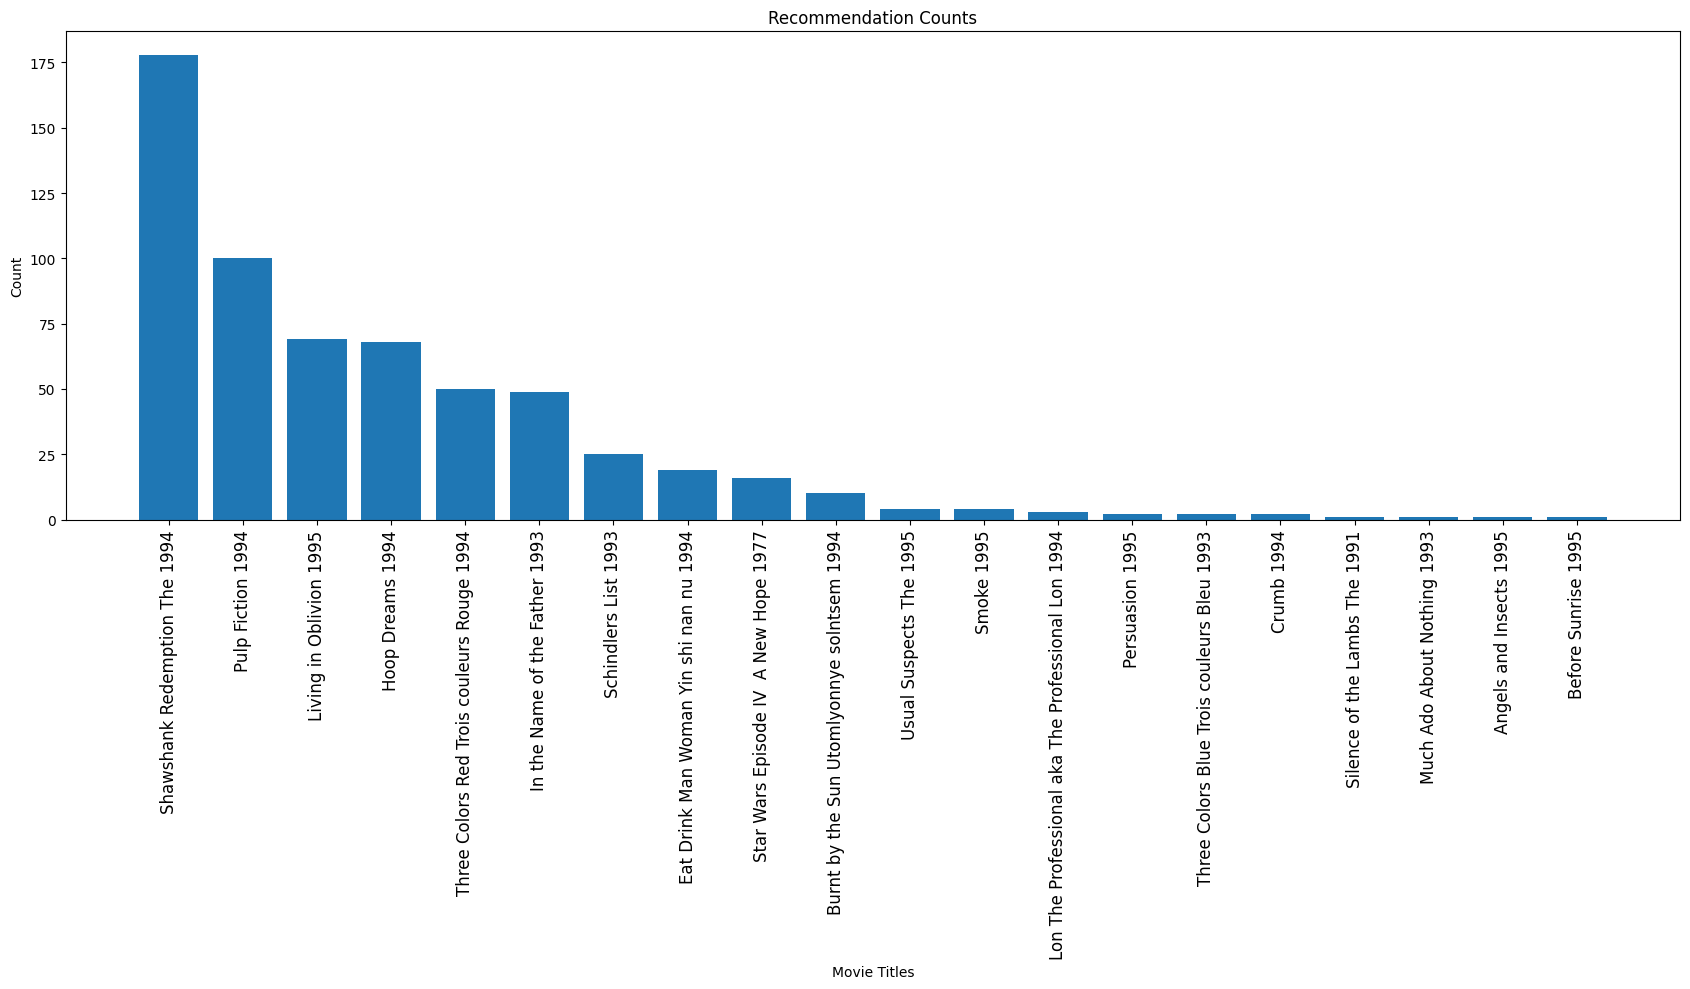
\includegraphics[width=0.9\textwidth]{colab_filter.png}
  	\caption{Top Recommendation of Movies}
  	\label{fig:top_recs_cf}
    \end{minipage}
\end{figure}

\subsection{Validation}

\subsubsection{Mean Square Error}

Because this model is able to produce predicted ratings, we are able to use mean square error to calculate model performance.  Because it would be too computationally expensive to test every single movie, we take a Monte Carlo approach towards this. We randomly select a user and from the users films, randomly select a movie they have seen. We then calculate the expected rating given our model to obtain the Mean Squared Error (MSE). This is repeated for 1000 movies

After conducting this 20 times, we get an average MSE of 0.9694. For reference, by just predicting the average rating, following the same process, we get an average MSE of 1.079. Therefore, it's slightly better than average, but only marginally. 

While the ability to output interpretable predict ratings is a nice benefit of this simple collaborative filtering system, it's not necessarily that useful. When evaluating recommended movies, the distinction between a movie rated 5.0 and one rated 4.8 is typically negligible to the viewer. Both ratings fall within a range of high satisfaction, rendering either outcome a success in the context of recommendations. Generally, the only thing that matters is whether or not a movie should or shouldn't have been recommended. If you liked the movie, then the recommendation worked. If you didn't, then the recommendation did not work. Therefore this becomes a binary classification problem.

\subsubsection{Binary Classification}

We will evaluate performance based on Precision, Recall, and Accuracy, That way, we can also compare the performance of the ProbS and HeatS models. For binary classification, we consider a rating to be positive if it is 4 or above. From our samples of reviews, we have a fairly balanced dataset with 48,580 positive reviews, and 52,256 negative reviews.

\begin{figure}[t]
  \centering
  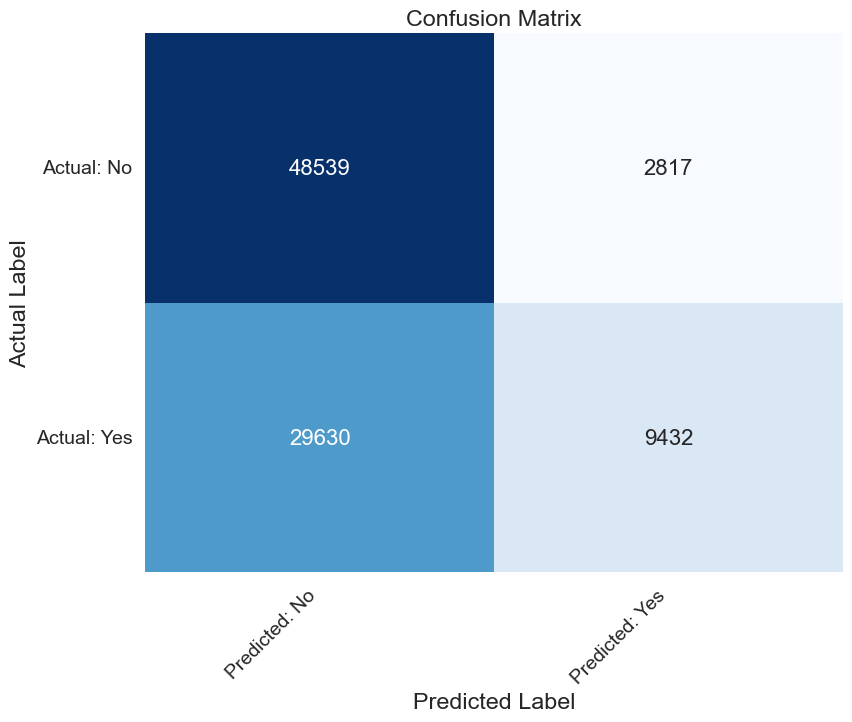
\includegraphics[width=0.5\textwidth]{conf_mat.png}
  \caption{Confusion Matrix with Collaborative Filtering}
  \label{fig:UN_degreeinfo}
\end{figure}

Figure 6.3 is the Confusion Matrix after running this with 90418 reviews. What we see is a huge imbalance towards predicting negative reviews. This results in an accuracy of 0.546, recall of 0.241, and precision of 0.770. In the evaluation of our recommendation system, precision takes precedence as a metric as it is much more important to only recommend movies that people enjoy rather than recommending all movies that a person would enjoy. Therefore, we see that even this simple Collaborative Filtering system beats ProbS, HeatS, and the baseline.

\section{Graphical Neural Networks}

Finally, we implement a Graphical Neural Networks (GNN) as recommendation system. In particular we use the architecture called LightGCN. This GNN is a simplified version of A Neural Graph Collaborative Filtering (NGCF), which adapts Graph Convolutional Networks in recommendation systems and employs one convolutional layer to exploit the direct connections between users and items \cite{lightgcn}. 

That is, LightGCN employs a simplified graph convolution that directly aggregates the embeddings of neighbour nodes without the use of transformation weights or non-linear activations, thus preserving the collaborative signal in the embeddings.

The embedding propagation can be recursively defined as:
\begin{align*}
	e_u^{(k+1)} &= \sigma \left( W_1 e_u^{(k)} + \sum_{i \in N_u} \frac{1}{\sqrt{|\mathcal{N}_u||\mathcal{N}_i|}} W_2 (e_i^{(k)} \cdot e_u^{(k)}) \right), \\
	e_i^{(k+1)} &= \sigma \left( W_1 e_i^{(k)} + \sum_{u \in N_i} \frac{1}{\sqrt{|\mathcal{N}_u||\mathcal{N}_i|}} W_2 (e_u^{(k)} \cdot e_i^{(k)}) \right),
\end{align*}
where $W_1$ and $W_2$ are trainable weight matrices, $\sigma$ denotes a non-linearity such as LeakyReLU, and $\mathcal{N}_u$ and $\mathcal{N}_i$ represent the sets of first-hop neighbors for users and items, respectively.

The user's final preference for an item is calculated using the dot product of the final user and item embeddings after $K$ layers of propagation, which are combined to obtain the final representations:
\begin{align*}
	\hat{y}_{ui} = (e_u^{(*)})^T e_i^{(*)}.
\end{align*}


\subsection{Model Architecture}

LightGCN simplifies the NGCF by removing feature transformation and non-linear activation steps. The architecture involves stacking multiple layers of simple weighted sum aggregators to capture the collaborative signal within the high-order connectivities.

The graph convolution operation in LightGCN is depicted as follows:
\begin{equation}
	e_u^{(k+1)} = \sum_{i \in \mathcal{N}_u} \frac{1}{\sqrt{|\mathcal{N}_u|}\sqrt{|\mathcal{N}_i|}} e_i^{(k)}
\end{equation}
\begin{equation}
	e_i^{(k+1)} = \sum_{u \in \mathcal{N}_i} \frac{1}{\sqrt{|\mathcal{N}_i|}\sqrt{|\mathcal{N}_u|}} e_u^{(k)}
\end{equation}
where $e_u^{(k)}$ and $e_i^{(k)}$ are the embeddings of user $u$ and item $i$ at the $k$-th layer, and $\mathcal{N}_u$ and $\mathcal{N}_i$ are the first-hop neighbors of user $u$ and item $i$, respectively.


The final embeddings are obtained by combining the embeddings from all layers. The user's preference for an item is predicted by the dot product of the user and item embeddings:
\begin{equation}
	\hat{y}_{ui} = (e_u^{(*)})^\top e_i^{(*)}
\end{equation}


The model employs Bayesian Personalized Ranking (BPR) loss, which is formulated as:
\begin{equation}
	L_{\text{BPR}} = -\sum_{u=1}^{M} \sum_{i \in \mathcal{N}_u} \sum_{j \notin \mathcal{N}_u} \ln \sigma(\hat{y}_{ui} - \hat{y}_{uj}) + \lambda ||e^{(0)}||^2
\end{equation}
where $\sigma$ denotes the sigmoid function and $\lambda$ is the regularization parameter. The model utilizes the Adam optimizer for training in a mini-batches.


\subsection{Implementation}

The implementation of the network is using an open source from Microsoft Recommenders (https://github.com/microsoft/recommenders), that is based in Pytorch. The parameters that we used was 3 layers, batch size of 1024, 1,000 epochs, a learning rate of 0.001 and we look for the top 10 most recommended movies. 

After training, we note that the networks converges as can be observed in the Figure \ref{fig:losses_over_epochs}. 

\begin{figure}[h]
	\centering
	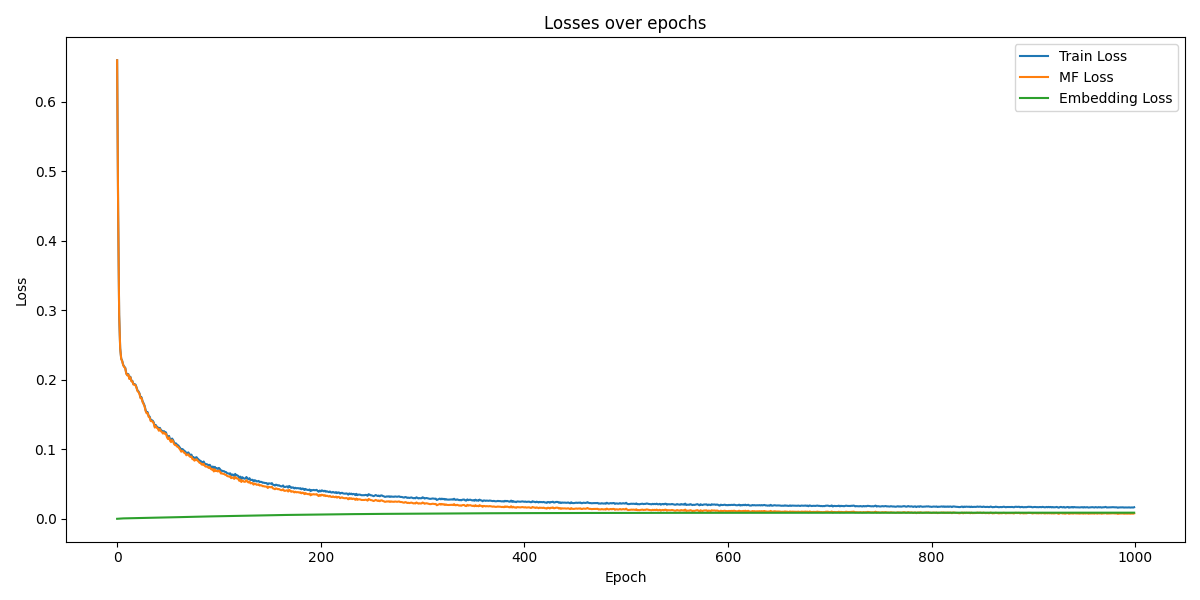
\includegraphics[width=0.8\textwidth]{losses_over_epochs.png}
	\caption{Convergence of the GNN.}
	\label{fig:losses_over_epochs}
\end{figure}

The code predicts the ranking of movies for every user instead of the rating itself like the last exercises. This ranking predicted is shown in the Figure \ref{fig:predictions}. 

\begin{figure}[h]
		\centering
	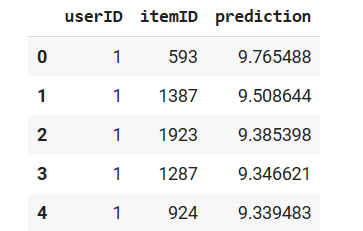
\includegraphics{predictions.png}
	\caption{Predicted Ranking for the user 1}
	\label{fig:predictions}
\end{figure}

With the top 10 scores predicted by the model, we evaluate how LightGCN performs on this test set. The metrics are in Figure 7.3.

\begin{figure}[!ht]
    \centering  % Centers the table
    \begin{tabular}{|l|r|}
        \hline
        \textbf{Metric} & \textbf{Value} \\
        \hline
        Precision & 0.277049 \\
        Recall & 0.162039 \\
        Mean Average Precision  & 0.203541 \\
        Normalized Discounted Cumulative Gain & 0.324148 \\
        \hline
    \end{tabular}
    \caption{Recommendation System Performance Metrics} % Add your caption
\end{figure} 

Figure 7.4 shows top 20 most recommend movies for all users. Similarly to CF, we get very famous movies, such as, Forest Gum, Matrix, Terminator, Lord of the Rings and Star Wars movies. 


\begin{figure}[h]
	\centering
	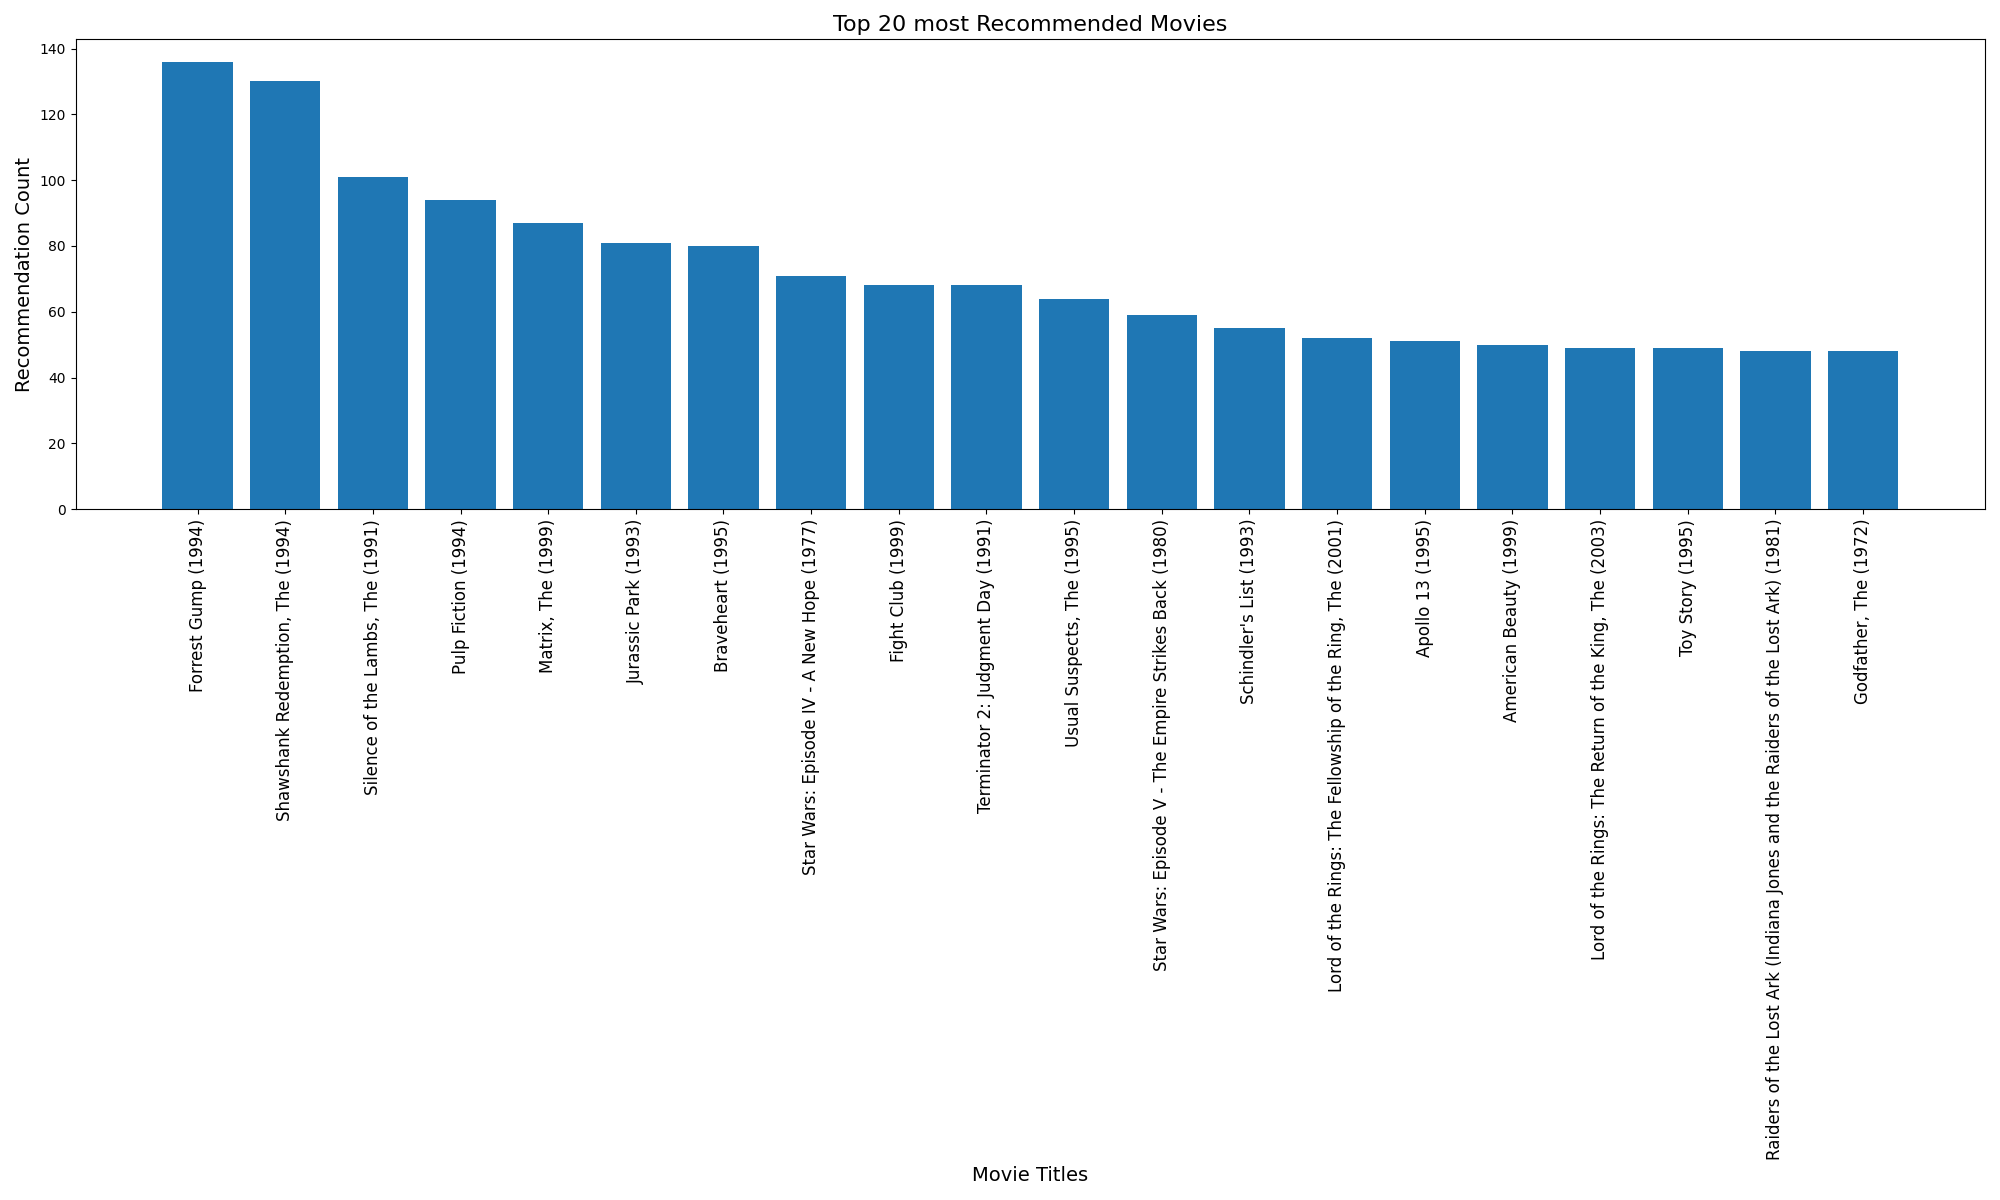
\includegraphics[width=1\textwidth]{top_20_movies.png}
	\caption{Illustration of user-item interaction and high-order connectivity.}
	\label{fig:top_20_movies}
\end{figure}

\newpage
\section{Conclusions}

Recommendation problems are often addressed using network analysis techniques, which involve constructing various types of graphs such as bipartite networks between users and items (e.g., movies) or weighted and unweighted directed graphs representing user similarity.

Further analysis involved examining the resulting networks, which were represented as adjacency matrices linking users to users and movies to other movies. 

Various approaches were explored for generating movie recommendations, by simplifying the problem as a binary classification methods with a focus on Precision and Recall mostly. Random Walk exhibited poor performance compared to simple average rating-based approaches, while collaborative filtering, which has been working for more than 30 years, showed the most promising results. One of the key challenges in recommendation systems is the "cold start" problem, where recommendations rely heavily on past user behaviour and struggle to provide accurate suggestions for new users or newly released movies.

To overcome these challenges, a GNN was implemented using PyTorch as a novel recommendation system. The model leveraged user and movie embeddings and employed a loss function that takes into account to user preferences. However, the results obtained were not superior to previous approaches. While GNNs hold promise, further refinement of the model architecture is necessary for improved performance.

The most effective recommendation systems often employ a combination of techniques. While collaborative filtering offers reasonable results, more sophisticated methods like Random Walk or GNNs can enhance predictions and address the cold start problem. By integrating diverse approaches, recommendation systems can achieve optimal performance and deliver personalized recommendations to users.


\vspace{1em} 




\newpage



\printbibliography

\end{document}